\RequirePackage{fixltx2e}
\documentclass[a4paper, titlepage, 12pt, twoside, open=right]{scrartcl}
\usepackage[utf8]{inputenc}  
\usepackage[T1]{fontenc}
\usepackage{mathtools}
\usepackage{longtable}
\usepackage{lmodern}           
\usepackage{polyglossia}
\usepackage{morewrites} %wtf
\usepackage{forest} % this is for the stemma diagram
\usepackage[onehalfspacing]{setspace}
\usepackage[toc,page]{appendix}
\usepackage{multirow,bigdelim}
\usepackage{parnotes}
\usepackage{xfrac}
\usepackage{graphicx}% stellt \scalebox bereit
\usepackage{array,booktabs}% für Tabellen
\usepackage{natbib}
\onehalfspacing
\setdefaultlanguage{english}
\usepackage{xeCJK}
 \setCJKmainfont[BoldFont=SimHei]{SimSun}
%\setCJKmainfont{Noto Sans CJK TC Regular}
\usepackage{marginnote}
\usepackage{geometry}           
\usepackage[multiple,perpage]{footmisc}
\usepackage{endnotes}
\def\enoteheading{\section{\notesname}%
\mbox{}\par\vskip-\baselineskip}
\geometry{left=2cm,right=3cm,top=2.5cm,bottom=2.5cm}
\usepackage{changepage}
\usepackage[hidelinks]{hyperref}
\usepackage{xcolor}
\usepackage{graphicx}
\usepackage{caption}
\usepackage{subcaption}

%avoid indent in quotes:
\makeatletter
\renewenvironment{quotation}
  {\list{}{\listparindent=1.5em
           \itemindent=0pt
           \parsep\z@ \@plus\p@}%
           \item\relax}
  {\endlist}
\makeatother


\begin{document}

\clearpage
\thispagestyle{empty}
\titlehead{}
\title{Through the Yellow Gate}
\subtitle{Ordination of Gender-Nonconforming People in Buddhism}
% \author{Ven. Vimala Bhikkhunī}
\author{DRAFT COPY}
\date{\today}
\maketitle

\newpage
\clearpage
\vspace*{200pt}


\begin{center}
\small I dedicate this work to my parents, who have raised me to see people as people, regardless of race, nationality, sex, gender or sexuality.
\end{center}

\newpage
\tableofcontents
\newpage
\section{Introduction}
Transgender and intersex people and at times other LGBTIQA+ have been excluded from ordination as a Buddhist monastic in the Theravāda tradition. This exclusion is the result of what I will show is an erroneous reading of several Pali terms--{\em paṇḍaka} and {\em ubhatob­yañ­janaka}--in the monastic disciplinary code (Vinaya Piṭaka) of the Theravāda school. Rendering the terms {\em paṇḍaka} and {\em ubhatob­yañ­janaka} into English, previous lexicographers of the Pali language have used vocabulary rooted in the Christian understanding of the early 20\textsuperscript{th} Century, like `eunuch' and `hermaphrodite'.\footnote{The Pali Text Society's Pali English Dictionary and Cone's Concise Pali English Dictionary. For dictionary entries I refer to \href{https://suttacentral.net/}{SuttaCentral.net}.} It has previously been noted that it is problematic to transpose Christian terms in the understanding and translation of other religious movements.\footnote{\cite{maes} page 2, \cite{dudas} page 45.} In dealing with the concepts of {\em paṇḍaka} and {\em ubhatob­yañ­janaka} the terms `eunuch' and `hermaphrodite', but also terms like `transgender' and `intersex' are inappropriate as they wrongly suggest that the lived understanding of the relationship between sex, gender and sexuality in Ancient India was the same as it is for us in the West today. The fact that certain groups of people are unable to obtain monastic ordination based on terms that are so little understood creates a barrier for all LGBTIQA+ people who come to Buddhism seeking refuge from suffering.

When studying the Buddhist scriptures, especially where there are groups of people who are marginalized, it is important to understand where and under which circumstances these concepts and interpretations have originated.
In the beginning of the Buddhist Order there were no rules for the conduct of monastics. The Vinaya was laid down later and grew as more rules were established. These were implemented only when monks started to misbehave and guidelines became necessary.\footnote{See Bhikkhu \cite{sujato2009} pages 8–10 for a more details on the context of the Vinaya.} The Vinaya as we have it today was formed over a long period of time and has been highly redacted over the centuries, regulating many and diverse aspects of monastic life. It is not an original Buddhist text that was passed down unchanged since the time of the Buddha. The oldest parts of the Vinaya consist of the rules ({\em pāṭimokkha}) and procedures ({\em kammavācā}), possibly together with some other materials. The different Vinayas in existence today are the products of the various schools of Buddhism that emerged much later.\footnote{After the Buddha passed away we see a gradual emergence of schools in the Aśokan and post-Aśokan periods. See Bhikkhu \cite{sujato2012} for a detailed study on the emergence of the Buddhist schools.} The Second Council is of preeminent importance in the development of the Vinayas as this is the only major event in Buddhist history that revolves entirely around a Vinaya dispute. Bhikkhu Sujato\footnote{See \cite{sujato2009} pages 141–142 and 215–216.} suggests that the bulk of the Vinaya texts were added well after the Buddha's death, in contrast to the Suttas: 

\begin{quote}
But the Vinayas were, it seems, composed following the Second Council; and in particular the {\em Khandhakas}, with their massive narrative arc, were put together in order to authenticate the acts of the Second Council.
\end{quote}

The Buddhist community also evolved in constant negotiation with its wider religious environment and needs to be understood as a dialogue with its various `religious others'. Claire Maes\footnote{See \cite{maes} and \cite{maes2016}.} has clearly demonstrated that this process was central to the formation of the Vinaya as an ongoing dynamic to create a distinctive Buddhist identity. The Second Buddhist Council became an important event in the history of Buddhism to determine its identity vis-à-vis other religious Orders after the Buddha passed away.

Many scholars have pointed out the many similarities between the principal practices, precepts and structures of Buddhists, Jains and Brahman communities and they seem to have had a detailed knowledge of each other's practices and organization.\footnote{See \cite{maes2016} page 9 footnotes 26–28.} The interaction and debates with these `religious others' led the Buddhist {\em Saṅgha} to implement specific rules in order to be in conformity with certain well-established monastic customs on the one hand and to (re)define their identity as a clearly separate Order on the other. In this paper I will argue that the concepts {\em paṇḍaka} and {\em ubhatob­yañ­janaka} have entered the Buddhist Vinaya after the Buddha passed away in the context of a much wider religious discussion that took place regarding the position of women within religious life that has also reduced the opportunities for women to ordain as Buddhist monastics.\footnote{The legality of the ordination of women ({\em Bhikkhunīs}) in the Theravāda and Tibetan lineages of Buddhism has been a hotly debated topic for many years. Thanks to the efforts and research of many monastics and academics, the first full Theravāda ordination was held in Perth in October 2009. Although still not widely recognized in several traditional Theravāda countries, recognition is growing and the number of Bhikkhunīs is slowly increasing. See a.o. Bhikkhu \cite{sujato2009} and Bhikkhu \cite{analayo2013} for research in this field.} 

I will also show that these terms have their roots in Vedic mythology and provide a fresh insight into the Asian paradigms for gender identities. Here we find the living proof of evolving ideas on sex, sexuality and gender that are very different from our Western concepts. And here we find that these terms are intimately bound up with the deeply ambivalent attitude towards women and women's sexuality in ancient India.

In this paper I will first trace the emergence of these--and other gender-specific--terms in Vedic, Brahmanic and Jain scriptures and their changes over the centuries. I will then discuss the occurrences of these terms in the Pali and Chinese Vinayas and compare these with the understanding of the contemporary `religious others' to come to a deeper understanding of what the terms {\em paṇḍaka} and {\em ubhatob­yañ­janaka} really meant at the time these passages were written and the reasons why these are said to be barred from ordination. Finally I will show that neither these terms, nor any other regulations in the Vinaya, can be used as a justification to exclude candidates from ordination based on their sex, sexuality or gender.
\section{Vedic, Brahmanic and Jain Scriptures}

Various authors have already noticed the similarities of Vinaya terminology between the Buddhist and Jain Orders.\footnote{See \cite{maes2016} page 9 footnotes 26–28, also \cite{sujato2009} and \cite{zwilling}.} In the Buddhist Suttas we find many examples of discussions between the two groups and after the Buddha passed away such discussions would certainly have had an impact on the Buddhist Vinaya. Both groups would have also used vocabulary that was already in existence at that time. It is therefore important to first have a look at what gender meant in the larger context of the society in pre-Buddhist India and how this understanding developed within the Jain Order.

\subsection{Emergence of the Third Gender}
We can trace the emergence of the concept of a third gender back to the late Vedic period (800–600 BCE). In the Vedic myths and legends, we frequently find the recurrent theme of a man turning into a woman or of being both a mother and a father. The function of these myths and legends is to confront deep anxieties and fears associated with the complex and problematic issues involving sex, gender, sexuality, power, hierarchy and subordination. We see literary representations of these anxieties in all patriarchal societies, expressing the deeply ambivalent attitude towards women and women's sexuality. On the one hand, women are depicted as pure and nurturing as long as they are controlled within the constraints of kinship, but outside such a regulated environment they are seen as dangerous and destructive to men. Through such projective devices of men onto women, male-dominated cultures have been able to establish a hegemonic ideology of gender.\footnote{See \cite{sujato2011} for an extensive work on the role of the male/female relationship portrayed in mythology in Buddhism and more specifically with regards to women's ordination.} We see that `transgenderism' is a recurring theme in these myths and legends, derived from these anxieties and attitudes towards gender.\footnote{\cite{goldman} gives an excellent account of the myths that formed the notions of gender in ancient India.}

The term {\em napuṃsaka} was originally an umbrella term used to denote men who were impotent, who had a female gender-expression or dressed in traditional women's clothing.\footnote{\cite{zwilling} page 362.} Literally the term means `not a male' i.e. men who did not conform to gender-role expectations. 

It is accepted by many scholars that the {\em hijras} of India are the contemporary representatives of these {\em napuṃsakas} and they even refer to themselves as `not a male' or `neither male nor female'.\footnote{See \cite{zwilling} page 363, \cite{goldman} page 388 and \cite{wendy}. A good study on the {\em hijras} is provided by Serena \cite{nanda}.} Although the {\em hijras} have been subject to influences from the Muslim period from the 12\textsuperscript{th} to the 16\textsuperscript{th} Century as well as from Christian and more modern Western ideas, by studying them we get a glimpse of what the lives of the {\em napuṃsakas} must have been like in Vedic times. 

The {\em hijras} are a representation of the god Śiva in their androgynous form of Ardhanārīśwara from Vedic mythology. They enact the religious myths and make them come alive in the rituals, songs and dances they perform. They are viewed as vehicles of the divine power of the Mother Goddess, which transforms their impotence into the power of creation. According to sources from the beginning of he 20\textsuperscript{th} Century, potential candidates for initiation as a {\em hijra} (which includes emasculation) had to be born impotent.\footnote{The 19\textsuperscript{th} and early 20\textsuperscript{th} Century sources are important because at that time the influence of globalization and the influx of Western ideas on the lives of the {\em hijras} was less prevalent as it is today. See \cite{ibbetson} pages 332, \cite{shah} page 1325 and \cite{bhimbhai}. Some 19\textsuperscript{th} Century accounts report that impotence was an essential qualification for admission into the hijra community and that a newcomer initiated into the community was on probation for as long as a year. During this time his impotence was carefully tested, sometimes by making the person sleep four nights `with a prostitute'. Only after impotence was established would the newcomer be permitted to undergo the emasculation operation and become a full member of the community. \cite{preston}.} Their emasculated body is not the only characteristic of a {\em hijra}, but also their physiology and their sexual capacities, feelings, preferences and behaviors. Although dressing like a woman is part of a {\em hijra}, they are also something quite different from a transgender person; they are the religious embodiment of the deities.\footnote{See \cite{nanda}.}

The adoption of the word {\em napuṃsaka} as a grammatical third gender\footnote{{\em Śatapatha Brāhmaṇa (ŚB) 10.5.1.2–3}.} in the 6\textsuperscript{th} Century BCE seems to have prompted a significant shift in meaning, because now the {\em napuṃsaka} was interpreted as meaning `neither male nor female'. This resulted in the previously mentioned `not males' to be regarded as persons with ambiguous gender.\footnote{See \cite{zwilling2000} page 362.} The individuals that the word {\em napuṃsaka} originally referred to were however all males, just not conforming to gender-role expectations. The word {\em napuṃsaka} itself retained its masculine form in grammar.

The fact that Sanskrit is a gendered language forced people to assign a gender to all objects including all living beings and humans. Gender was seen as a property belonging to objects and objects are gendered by the presence or absence of certain defining characteristics or {\em liṅga}.\footnote{The original meaning of {\em liṅga} is `characteristic mark or sign' (Nirukta 1.17) but it later starts to mean `sexual characteristic'. See also chapter \ref{linga} for a detailed description of {\em liṅga}.} The third gender ({\em napuṃsaka}) was basically a class for things that were neither male nor female in nature. This meant that there was an intimate connection between sex and grammatical gender that had far-reaching consequences and caused much confusion.\footnote{Other languages, like the Uralic languages, do not have gender in language. Such gender-less languages exclude many possibilities for reinforcement of gender-related stereotypes as they do not place objects (and thus people) in boxes.} 

Just after the late Vedic period we see that a set of terms relating to the class of {\em napuṃsakas} emerged like {\em klība} (sexually defective man\footnote{As pointed out by \cite{zwilling} page 363, the nature of the {\em klība} is suggested by the Bṛhadāraṇyaka Upaniṣad 6.1.12 and can be acquired due to the destruction of the penis as in ŚB 1.4.3.19.}) and {\em paṇḍaka} (`impotent', or `sterile'\footnote{Atharva Veda (AV) 8.6.7, 11.16. The etymology of {\em paṇḍaka} is unknown but cf. baṇḍa at AV 7.65.3 is glossed by the commentator as {\em nirvīrya} (`impotent'). Albrecht \cite{wezler} has suggested that paṇḍa and paṇḍaka be regarded as ultimately derived from {\em *apa}+ {\em āṇḍā}, thus: “one who has no testicles (anymore),” i.e. a eunuch. Allan \cite{bomhard} points out that there is a range of translations and interpretations that can apply to the {\em paṇḍaka}. He believes that the word can be a loan-word from the Dravidian {\em peṇṭan, peṇṭakan, peṇṭakam}, which can mean both hermaphrodite and eunuch.}). Both of these types were associated with cross-dressing and dancing, as we have also seen in the above description of the contemporary {\em hijras}. With the word {\em napuṃsaka} having gained a much broader meaning, it seems likely that these new sub-categories represent different names for the original meaning of `not males'.

\subsection{Sex and Gender in the Jain Order}
Just like in Buddhism, the Jain Order had a strong interest in controlling the sexuality of its monastics. Jain monastics practiced celibacy, and the monks were mostly naked ascetics. The prestige and power of the Order depended to a large extend on public opinion and therefore on the purity of their behavior, as well as their external appearance. The `third gender' was therefore the subject of a very lengthy debate within the Order. 

In addition to these practical considerations, there was also a debate within the Jain community as to whether women can attain spiritual liberation because the monks felt it was improper for them to go naked. Eventually it was this dispute that led to the schism between the two major Jain Orders.\footnote{See Paul \cite{dudas} for an extensive account of the schism. The two main sects of Jainism, the {\em Digambara} and the {\em Śvētāmbara} sects, likely started forming about the 3\textsuperscript{rd} Century BCE and the schism was complete by about 5\textsuperscript{th} Century CE.} This controversy hinged on the identification of the signs to designate somebody as a woman, which logically also led to the examination of what is male, and `neither male nor female'. 

The speculations and discussions that followed focused on the characteristics necessary to identify a person as belonging to one of three groups. The {\em paṇḍaka}, {\em klība} and {\em keśavan} (long-haired male)\footnote{Apparently long hair was seen as a sign of a woman.} were recognized as males, but their gender-role nonconformity assimilated them to females, so not `real males' and therefore still {\em napuṃsakas}. Yet their grammatical gender was masculine.

This discussion was influenced by the Brahmanical views at that time concerning the essential markers for gender assignment ({\em liṅga}).\footnote{I will discuss the meaning of this term in more detail in chapter \ref{linga}.} By the 3\textsuperscript{rd} Century BCE two views had developed to define gender.

\begin{enumerate}
 \item The first view went from the premise that gender was defined by what one perceived as a man, woman or neither based on the presence or absence of primary or secondary characteristics.\footnote{Mahābhāṣya 4.1.3: Q: ``What is it that people see when they decide, this is a woman, this is a man, this is neither woman nor man?'', A: ``That person who has breasts and long hair is a woman; that person who is hairy all over is a man; that person who is different from either when those characteristics are absent, is {\em napuṃsaka}.''}
 \item The second view is that gender assignment has to do with the ability to procreate or conceive. 
\end{enumerate}

Both these Brahmanical views were rejected by the Jains as being inadequate to determine gender. Paul \cite{dundas} describes how the Jains developed a system to define gender as a combination of sex, behavior, physical characteristics and also the underlying sexuality and feelings. The Jains came up with their own term {\em veda} to describe these characteristics.\footnote{This move is rather remarkable because for the Brahmins {\em veda} meant their sacred knowledge and scriptures. But it is not unprecedented because the Jains often used existing words and gave them new meaning. In the Buddhist Suttas we also find instances where the Buddhists use different terms for the same things as the Jains. F.i. Majjhima Nikāya 56 recounts a discussion between the Buddha and the Jain ascetic Tapassī in which the ascetic mentions that their leader Nigaṇṭha Nātaputta {\em (i.e. Mahāvīra)} doesn’t speak in terms of ‘deeds’, like the Buddha, but uses the term ‘rods’.” See also \cite{zwilling} note 34.} This conception of sexuality most likely predates the schism between the two major Jain sects but was not part of the earliest Jain doctrine. This concept appears frequently in the later canonical Jain texts but is also mentioned once in the early Jain literature where male sexuality is explained as sexual desire for women and female sexuality is explained as sexual desire for men.\footnote{See {\em Viyāha 2.5.1}.} The sexuality of the {\em napuṃsaka} is not clearly defined in the earlier texts but is seen as a threat to the chastity of monks.\footnote{See Ācārāṅga Sūtra (English translation by \cite{jacobi}) p.220: monks are warned that a danger of drunkenness is seduction by a woman or a {\em klība} page 285: sleeping places frequented by women or {\em paṇḍakas} are to be avoided.}

Zwilling and Sweet\footnote{See \cite{zwilling} page 368.} mention:

\begin{quote}
... we may infer that sexual desire for a man forms at least one aspect of third-gender sexuality. In a set of similes descriptive of the relative intensities of the sexualities of the three gender, that of the third gender is viewed as most intense of all: a woman's {\em veda} is compared to a dung fire, a man's to a forest fire, but the third gender's is compared to a burning city. Thus third-gender persons are not only sexual persons, but hyperlibidinous ones at that.
\end{quote}

The word {\em napuṃsaka} has been the subject of much debate within the Jain Order, resulting over time in changes in meaning and use and the definition of sub-categories. The word in the canonical texts seems to have referred only to males who were cross-dressing and had a female gender-expression, who are identified by the way they dress, their behavior and sexual orientation. Because they looked like a woman, they were also assumed to have sexual desire for men. Because of this characterization, the {\em napuṃsaka} can also be an object of lust for celibate monks and would have been seen as problematic for ordination as a male monastic. Part of the discussion was also fuelled by the nakedness of the Jain monks and therefore their physical male appearance as well as their behavior. As celibate monks, same-sex relations and the possibility of same-sex attractiveness were also an issue. The public perception, and the fear thereof, was of utmost importance for the livelihood of the Jain Order. 

We also see a shift in the discussion over time regarding the abilities of a {\em napuṃsaka}, or at least some sub-categories thereof, to attain enlightenment or to ordain. The {\em Śvētāmbara} in their later Bhāgavatī Sūtra\footnote{Bhāgavatī Sūtra 4.1–2.} even define a fourth gender, namely the {\em puruṣanapuṃsaka} (male {\em napuṃsaka}, possibly a {\em napuṃsaka} who appeared the same as other men).\footnote{see \cite{zwilling} for more details.} Lacking any of the external characteristics of a {\em napuṃsaka}, the only characteristic left to define them as such must have been their sexuality (i.e. attraction to men).

During the period of the commentarial literature the sexuality of the {\em napuṃsaka} was redefined as being of a more bisexual orientation. Leonard Zwilling and Michael Sweet\footnote{See \cite{zwilling} pages 371–374.} believe that this new definition was not so much driven by actual observations of the behavior of {\em napuṃsakas} but rather by theoretical discussion. This bisexual orientation was not conceived of as a separate orientation, but as possessing the sexuality of \textbf{both} males and females. This is a change from the canonical literature, where the sexuality of a {\em napuṃsaka} was characterized as female only.

During the period in which the commentarial literature was established the terms male and female {\em napuṃsaka} were redefined further. The female {\em napuṃsaka} was the old category defined in the Canon of which the {\em klība} and {\em paṇḍaka} are sub-categories, and the male {\em napuṃsaka} was the aforementioned {\em puruṣanapuṃsaka}. The female {\em napuṃsaka} seems to act as a female partner only (i.e. be acted upon), while the male {\em napuṃsaka} acts in both ways. So here male and female sexuality are no longer just defined as the sexual desire to have sex with a female and male respectively, but also in terms of the role taken in intercourse.\footnote{Niśītha Sūtra 3507.} The hyperlibidinous nature of the {\em napuṃsaka} was ascribed to the bisexual character of his sexuality.

It is interesting to note that throughout this discussion the {\em napuṃsaka} and its sub-categories always refer to males who are somehow blocked in terms of exercising their male sexuality in one way or another owing to their performance of some unvirtuous act (karma) in a previous life. Females who did not conform to gender-expectations were not considered in the class of {\em napuṃsakas} or are only very rarely mentioned, without much explanation as to their nature. 

\subsection{Jain Monastic Ordination}
In the formative years of the Jain Order, the rules for ordination were still rather simple. Only the {\em klība}, the {\em paṇḍaka} and ill people were not allowed to ordain. Of the two Jain sects after the schism, the {\em Digambara} maintained nakedness and eligibility to ordain as a monk was quite straightforward: one had to be a man without genital defects and virile, except for when that man was overly libidinous. 

For the {\em Śvētāmbara}, who wore a cloth, the matter was far more complex and they devised an intricate system of people suitable for ordination, whereby the {\em napuṃsaka} was divided into sixteen types.\footnote{See Bhagavatī 5166–67.} Over time, the ban against ordination of {\em napuṃsakas} was relaxed, first based on practical grounds like a known and well-behaved candidate, and later an exception was made for those who were able to control their sexuality. One of the main grounds why certain {\em napuṃsakas} were denied ordination was their perceived hyperlibidinous-ness, which would render them incapable of keeping their vows of celibacy and made them unfit to live in either the monks' or nuns' communities. Only ten of the sixteen were not allowed to be ordained because they were regarded as uncontrollable in their passions. Among these were the original two categories of {\em klība} and {\em paṇḍaka}. The aforementioned {\em puruṣanapuṃsaka} was allowed to ordain, presumably because they could not potentially evoke a monk's lust. Since external appearance was no longer a clear guide to who is {\em napuṃsaka}, the candidate for ordination had to be questioned. 

By the 17\textsuperscript{th} Century CE, this rule on ordination had been nearly abolished. So we have seen a radical shift from total non-acceptance to almost total acceptance of {\em napuṃsakas} in the Jain Order over time.\footnote{\cite{zwilling} references {\em Yuktiprabodha} in footnote 80.}


\section{Liṅga and the Dispute on Women's Ordination}
\label{linga}

As we have touched upon in the context of the developments in the Jain order there was a lively discussion around the 3th century BCE on what the characteristics of sex or gender are. This controversy hinged on the identification of the signs to designate somebody as a woman, which logically also led to the examination of what is male, and 'neither male nor female'. This was a much wider religious debate that involved both the Jain and Buddhist communities as well as possible other sects. Bhikkhu Sujato\footnote{See \cite{sujato2009} page 241–242.} points out that these discussions were held amongst the monks, while the women themselves were notable by their absence. We have no indication that this was any different in the Jain order. It is therefore not surprising that at the Second Buddhist Council, which was held at around the same time, rules were laid down with regards to the ordination of nuns, and most likely the 'third sex' category, with it's perceived hyperlibidinous-ness, was also touched upon. We also find for instance various passages with regards to women's role in the order that seem out of place in the Buddhist scriptures but which use near identical wording in the Jain texts\footnote{See \cite{sujato2009} page 54–55.} so it is clear that there was a distinct influence between the orders.

This discussion regarding {\em liṅga} in the light of ordination into the Buddhist monastic order is all the more remarkable because monks and nuns forego the usual markers of sex and gender when they put on robes and shave their heads. Giving up gendered attire is one of the distinguishing characteristics of monastic life. In the Jain order this discussion made more sense\footnote{\cite{maes2016} pages 11–17 points out that the Jain's nakedness was one of the primary distinctive marks that set them aside from Buddhist monastics. The wearing of a bowl and robe was an important part of the Buddhist identity.}. The Jain were naked ascetics and therefore the physical marks of sex could not so easily be given up. The women needed to wear a cloth to cover their bodies while the men could go naked. This was a very important point for the Jain because this difference also meant that as women could not let go of all earthly possessions they could also not reach enlightenment. This was one of the main points of dispute between what became the two sects in Jainism.

The original meaning of the term {\em liṅga} before this dispute is 'characteristic mark or sign'\footnote{Nirukta 1.17. Also used in the early Buddhist Suttas in this way, f.i. Majjhima Nikāya 98 Vāseṭṭhasutta.}, but during this dispute the term was refined and the different orders developed different opinions about the characteristics of 'male' and 'female'. In the Buddhist Abhidhamma the term is often referred to exclusively as denoting sexual characteristics. Burkhard Scherer\footnote{\cite{scherer} page 68.} takes the term {\em liṅga} as a reference to the 'secondary sex organs' or characteristics of sexual difference, which also include behavioral differences so the term can be used to denote both biological sex and gender-identity as we define it today. He bases this conclusion on the work of Buddhaghosa, who listed the secondary characteristics of the male and female, which included beards and moustaches, motherly instincts, way of walking, etc. This is also in line with the first Brahmanical view on this matter as well as what is described in the Buddhist {\em Abhidharmakośa}\footnote{Abhidharmakośa IV.14 c. using the word {\em vyañjana} as a synonym for {\em liṅga}.}, the {\em Samantapāsādikā} commentary\footnote{See \cite{anderson2016} page 237–240 for an English translation of the passage on change of {\em liṅga} in a monastic.} and elsewhere. There is no indication that the Buddhists agreed with the Jains on the inclusion of underlying sexuality and sexual feelings in the definition of {\em liṅga}\footnote{The Jain also defined the sexual desire for the male body as part of the female characteristics and visa versa.}.

This change of meaning in the word {\em liṅga} has caused a lot of confusion and is especially important in determining the characteristics of the {\em paṇḍaka} and {\em ubhatob­yañ­janaka} in the next chapters.\\
\\
In the next chapters I will discuss the various terms and their occurrences in the Buddhist canon. A listing of the occurrences of the most common terms pertaining to gender like {\em paṇḍaka} and {\em ubhatob­yañ­janaka} in Chinese texts is given in Appendix \ref{appendix1}. 

\section{The Paṇḍaka}

\subsection{The Paṇḍaka in the Pali Vinaya}
In the Theravāda Vinaya the term {\em paṇḍaka} is mainly used in the context of individuals a monastic should not have sexual relations with or as a form of insult. The rule regarding the ordination of {\em paṇḍakas} is laid down in {\em Khandhaka 1}\footnote{Khandhaka 1 Pabbajjā PTS vol 1 page 85–86.} and reads as follows\footnote{Translation by Ajahn Brahmali.}:

\begin{quote}
{\em Tena kho pana samayena aññataro paṇḍako bhikkhūsu pabbajito hoti. So dahare dahare bhikkhū upasaṅkamitvā evaṃ vadeti—“etha, maṃ āyasmanto dūsethā”ti. Bhikkhū apasādenti—“nassa, paṇḍaka, vinassa, paṇḍaka, ko tayā attho”ti. So bhikkhūhi apasādito mahante mahante moḷigalle sāmaṇere upasaṅkamitvā evaṃ vadeti—“etha, maṃ āvuso dūsethā”ti. Sāmaṇerā apasādenti—“nassa, paṇḍaka, vinassa, paṇḍaka, ko tayā attho”ti. So sāmaṇerehi apasādito hatthibhaṇḍe assabhaṇḍe upasaṅkamitvā evaṃ vadeti—“etha, maṃ āvuso dūsethā”ti. Hatthibhaṇḍā assabhaṇḍā dūsesuṃ. Te ujjhāyanti khiyyanti vipācenti—“paṇḍakā ime samaṇā sakyaputtiyā. Yepi imesaṃ na paṇḍakā, tepi ime paṇḍake dūsenti. Evaṃ ime sabbeva abrahmacārino”ti. Assosuṃ kho bhikkhū tesaṃ hatthibhaṇḍānaṃ assabhaṇḍānaṃ ujjhāyantānaṃ khiyyantānaṃ vipācentānaṃ. Atha kho te bhikkhū bhagavato etamatthaṃ ārocesuṃ. “Paṇḍako, bhikkhave, anupasampanno na upasampādetabbo, upasampanno nāsetabbo”ti.}
\end{quote}

\begin{quote}
At one time a certain {\em paṇḍaka} had gone forth as a monk. He approached the young monks and said, “Venerables, come and have sex with me.” The monks dismissed him, “Go away, {\em paṇḍaka}. Who needs you?”

He went to the big and fat novices, said the same thing, and got the same response.

He then went to the elephant keepers and horse keepers, and once again he said the same thing. And they had sex with him. They complained and criticized them, “These Sakyan ascetics are {\em paṇḍaka}s. And those who are not have sex with them. None of them is celibate.”

The monks heard their complaints. They told the Buddha and he said, “A {\em paṇḍaka} should not be given the full ordination. If it has been given, he should be expelled.”
\end{quote}

There are a couple of interesting things to note about this passage. First of all, the {\em paṇḍaka} in question was already ordained at the time of this incident. The rule against ordination of the {\em paṇḍaka} clearly mentions that full ordination of these individuals, the {\em upasampadā}, is not allowed. This really only makes sense if we understand {\em pabbajjā} here to be equivalent to {\em upasampadā}. In fact this equivalence between {\em pabbajjā} and {\em upasampadā} is what we find throughout the earliest Vinaya, and indeed the suttas \footnote{The {\em sāmaṇeras/īs} are barely mentioned in the suttas. Instead we find the figure of the {\em samaṇuddesa}, 'one designated as a {\em samaṇa}', who seems to have had a looser affiliation with the Sangha, that is, no proper ordination. The commentaries glosses them as {\em sāmaṇeras}, but this might be an oversimplification. More likely they were a kind of precursor to the more formal status of novice. It seems likely that such people merely put on robes, and then lived in with loose connection to a particular community of ascetics, in which case their sex would have been a non-issue. I would argue it is natural to see novices proper in the same way. But the {\em samaṇuddesa} remains obscure.}. In any case, the rule itself is clearly limited to {\em upasampadā} (full ordination) and novice ordination seems to be allowed.

The Theravāda commentary, both in regards to the {\em paṇḍaka} and the {\em ubhatob­yañ­janaka} differs from the Vinaya in making a distinction between {\em pabbajjā} (in the meaning of novice ordination) and {\em upasampadā} (full ordination) and does not allow either for ordination.

A second interesting point is that the monks and novices that are approached by the {\em paṇḍaka} react in an exemplary manner and send him away. It is only the elephant and horse keepers, those of a lower class, who engage in sexual relations with him. But afterwards, they still complain about it and criticize the {\em paṇḍaka} while they have themselves also engaged in the same act. This seems a bit odd and revolves around the stock passage {\em Te ujjhāyanti khiyyanti vipācenti} that is used throughout the Vinaya as a typical pattern of narration. In the majority of cases it is the {\em manussā} (people) who complain and criticize, after which the monks hear about it, also complain and criticize ({\em Ye te bhikkhū appicchā …pe… te ujjhāyanti khiyyanti vipācenti}) and then relate the story to the Buddha. So the word {\em te} (they) is used to relate to the monks who criticize after they have heard it from the 'people'. Here however the word {\em te} is used right after the elephant and horse keepers, seemingly referring to them. However, it would make much more sense if others would complain about this scandalous behavior rather than the elephant and horse keepers themselves. Indeed this is what we find in the same story in the Dharmaguptaka Vinaya, where the people (lay Buddhists) complain and criticize (時諸居士見已譏嫌言). Claire Maes\footnote{See \cite{maes2011} pages 98–101.} points out that this phrase could have been used to conceal debates that might have influenced the Bhikkhu Sangha to implement specific precepts to be in conformity with the praxes of other ascetic communities with the main purpose to place the origin of precepts within the Buddhist Order with the Buddha himself in a leading role. She successfully demonstrates this with the Jain concept of {\em ekindriya jīva} (one-facultied life) and argues that this concept entered the Buddhist Vinaya as a result of interactions and discussions with the Jain contemporaries. I believe that the {\em paṇḍaka} could also have entered the Buddhist Vinaya in a similar manner. As we have seen previously, the {\em paṇḍaka} was discussed at length in the debate amongst the Jains themselves.

In Appendix \ref{appendix2}, figures \ref{pali1} and \ref{sanskrit1} I have charted the occurrences of the various words throughout the Pali and Sanskrit texts. This illustrates that the {\em paṇḍaka} only occurs in the Vinaya and Commentaries in the Pali. The Sanskrit texts in this graph are not entirely organised by lateness but it is clear that the {\em paṇḍaka} mainly appears in the Vinaya and {\em Śāstrapiṭaka}. The {\em klība} is notable by it's absence in all Buddhist texts and only appears in the Vedic and later Brahmanical texts. It does not appear in the Pali texts at all. One explanation for this might be that the terms {\em klība} and {\em paṇḍaka} have been mixed up because their meanings were at least in part overlapping. What is also striking is that the umbrella term {\em napuṃsaka} only appears in the Pali commentarial texts and not in any of the earlier collections. It is however a recurrent term in the Vedic and Brahmanical texts. We also see that this term becomes more prominent in the later Anya commentaries as well as in the Brahmanical {\em Śāstra} collections, which points to a shift in emphasis, and possibly meaning, of this term in later times at the expense of the prominence of {\em paṇḍaka}. As these are later texts I have not looked into them in great details and this might be an interesting topic for later studies.

Considering that the word {\em paṇḍaka} does not appear in any of the early suttas\footnote{The word is not found in any of the early Buddhist Suttas, nor does it appear in the {\em pātimokkhas}, the lists of rules for monastics. Next to the Pali Vinaya, it appears twice in the {\em Aṅguttara Nikāya}, but both of these only have parallels to the Vinaya or later texts.}, it seems clear that the inclusion of the word in the Vinaya did not happen in the Buddha's lifetime but was added later as a result of the discussions with the Brahmins and Jains, for whom the {\em paṇḍaka} could not ordain.

\subsection{The Five Types of Paṇḍaka}
Going beyond the Vinaya itself into the commentarial scriptures, we find the following in the Theravāda {\em Mahāvagga-aṭṭhakathā} to explain more about the nature of these two classes\footnote{The {\em Samantapāsādikā}: Vol. V, p. 1015f. is a translation of Sinhala commentaries into Theravāda by Bhikkhu Buddhaghosa and possibly others in the 5th century CE. It was based on the Mahāpaccariya and the Kurundī Atthakathā. See \cite{goonesekere} for details on Theravāda Commentaries.}. It defines five types of {\em paṇḍaka}\footnote{Translations/explanations as in \cite{bomhard} and \cite{thanissaro}.}:

\begin{enumerate}
\item {\em āsittapaṇḍaka}: a man who gains satisfaction from performing oral sex on another man and from swallowing his semen or who only becomes sexually aroused after swallowing another man’s semen. 
\item {\em usūyapaṇḍaka}: a voyeur, that is, a person who gains sexual satisfaction from watching others have sex. 
\item {\em opakkamikapaṇḍaka}: eunuch, due to castration.
\item {\em pakkhapaṇḍaka}: those who become sexually aroused in parallel with the phases of the moon\footnote{According to \cite{bomhard}, the term pakkhapaṇḍaka (Skt. {\em pakṣapaṇḍaka}) probably does not refer, as traditionally understood, to an individual who becomes sexually aroused parallel to the phases of the moon, i.e., to someone who is aroused during the fortnight of either the waxing or waning moon, but to someone “who acts wrongly sexually, who behaves badly sexually.” He hypothesizes that {\em pakkha} of the compound {\em pakkhapaṇḍaka} should be understood in terms of its alternative meaning “a cripple,” and that the corresponding Sanskrit should not be understood as {\em pakṣa} but rather {\em phakka} (“cripple,” adj. “lame, crippled, maimed”), derived from the Skt. verbal root {\em phakk}, (a) “to creep, to steal along; (b) to have a preconceived opinion; (c) to act wrongly, to behave badly.” He thus considers the third meaning of phakk as most relevant to the case at hand.}.
\item {\em napuṁsakapaṇḍaka}: a person born without sexual organs\footnote{The Sanskrit equivalent is {\em prakṛtipaṇḍaka}. The term {\em prakṛti} means something like 'nature' or 'fundamental form' and the term {\em tṛtīyāprakṛti} became the official word for the 'third sex' at around the beginning of the common era. I therefore do not believe this translation by \cite{thanissaro} to be correct but that the literal meaning reflects more the original meaning of {\em napuṁsaka}.}. 
\end{enumerate}

It is interesting to note that not all {\em paṇḍaka} are barred from ordination, in contrast to what the Vinaya mentions. Only the last three types are forbidden to ordain\footnote{\cite{wong} and \cite{thanissaro}.}.

The castrated {\em paṇḍaka} i.e. a eunuch, is only one of the five types that cannot ordain, which makes it highly unlikely that the word {\em paṇḍaka} means 'eunuch'. We would also not expect a eunuch to have hyperlibidinous-ness. After all, castrated men were often employed as harem guards just for the reason that they are no longer interested in sexual activity and therefore considered safe. Moreover, the Dharmaguptaka Vinaya treats the castrated man as something other than a {\em paṇḍaka}.

As we have seen in the Jain scriptures, the discussion to overcome the ambiguities in the understanding of the word {\em napuṁsaka} resulted over time in changes in meaning and the definition of sub-categories and I believe this has also occured in the Buddhist Vinayas with the word {\em paṇḍaka}. I believe that it is likely that the term {\em opakkamikapaṇḍaka} represented a castrated man, the {\em klība}, while the {\em napuṁsakapaṇḍaka} was the re-definition of the original {\em paṇḍaka} or the 'female {\em napuṃsaka}' that we saw emerging in the Jain commentarial texts. Also from the Chinese sources it is clear that the person has to be born this way.

The {\em pakkhapaṇḍaka} is interesting and several explanations have been given by authors over time, none of which I find convincing. Allan \cite{bomhard} advocates that the word {\em pakkha} should not be translated as 'half moon' but that the meaning of the word is something like a sex-addict. I refute this argument because the characters used to denote this type of pandaka in the Chinese Vinayas of all schools are 半月, which literally means 'half moon'. It is also mentioned in various Chinese commentarial texts\footnote{f.i. X44 0744 0432c17 四分律名義標釋.} that the 'half moon' is 'not a male' and thus a form of {\em napuṃsaka} for half of the month and the other half he is a male. All texts are consistent in this. As we can still understand the meaning of the other four categories and understand their meaning in light of people's physiology or sexual fetishes, the 'half-moon' {\em paṇḍaka} is an enigma. Turning back to the Vedic texts however, we find in the {\em Uttarakanda} of the {\em Rāmāyaṇam}\footnote{Rām 7.78–79. See also \cite{goldman} page 379–380.} the story of King Ila. In this epic tale the king accidentally stumbles upon the Goddess Pārvatī in intimate embrace with Śiva, who turn him into a woman. Now Ilā, she turns to the Goddess for mercy to restore her manhood but is only granted half her wish; namely that she has to change sex each month. The theme of changing genders based on the phases of the moon is a recurrent theme in the Vedic myths and it is not unlikely that this mythical theme has found its way into the Vinaya in the form of the {\em pakkhapaṇḍaka}. After all, another rule in the Vinayas of all the schools tells the tale of a shape-shifting serpent, a mythological beast, a {\em Nāga}\footnote{Khandhaka 1 Pabbajjā PTS vol 1 page 86–88.}, who ordains as a monk, is later discovered and a new rule is laid down in much the same manner as for the {\em paṇḍaka}, barring him and all his kind from ordination. The fabric of myth and reality can easily overlap in Indic culture. The Vinaya is full of various strange and wonderful beings. The ­{\em Bhikkhu Pā­rāji­ka} 1, the rule against sexual intercourse, mentions that a monk is not allowed to have sex with a list of beings, namely a dragon, a spirit, a ghost and a {\em paṇḍaka}\footnote{PTS vol. 3 page 37: {\em Tena kho pana samayena aññataro bhikkhu nāgiyā methunaṃ dhammaṃ paṭisevi … yakkhiniyā methunaṃ dhammaṃ paṭisevi … petiyā methunaṃ dhammaṃ paṭisevi … paṇḍakassa methunaṃ dhammaṃ paṭisevi. Tassa kukkuccaṃ ahosi … pe … “āpattiṃ tvaṃ, bhikkhu, āpanno pārājikan”ti.}}. The fact that the {\em paṇḍaka} is listed in a list of mythological beings is indicative of its origins and how they were viewed at that time. We find similar lists in the Vinayas of the other schools.

As for the other two, the {\em āsittapaṇḍaka} and the {\em usūyapaṇḍaka}, who at least in the Theravāda tradition are allowed to ordain, I believe they embody another of the Jain categories, namely the category of the {\em puruṣanapuṃsaka} (male {\em napuṃsaka}). Although they might be impotent and are therefore also in possession of the female {\em veda}, their appearance is male to the lay supporters but also to the celibate monks they live with who are not aroused by their presence. The relaxation of the rules for these two types also runs parallel with the development in the Jain scriptures. But unlike the Jain, no further abolishment of this entire rule against the ordination of {\em paṇḍaka} was reached simply because the Buddhist scriptures were closed while the Jain scriptures continued to evolve for many centuries thereafter.


\subsection{The Paṇḍaka in the Chinese Vinayas}
The first thing that is striking when comparing the various Chinese schools is that there is no clear consistent term that denotes the {\em paṇḍaka}. The Mahāsaṅghika and Sarvāstivāda Vinaya use the term 種不能男 (impotent lit. incapable of producing seed) in the descriptions in the first Khandhaka on ordination. In the Dharmaguptaka Vinaya this term is only used in the description of the 'half-moon' {\em paṇḍaka}. The term 黃門 ('eunuch') is used in the Dharmaguptaka and Mahīśāsaka Vinaya while in the Sarvāstivāda Vinaya the term is used everywhere but in the ordination Khandhaka. As both the terms 種不能男 (impotent) and 黃門 ('eunuch') are used in the same way in different schools, we can assume that both can denote {\em paṇḍaka} but that the difference in terms point to historical changes in understanding and translation\footnote{Shinsan text X44 0744 0432c13 (四分律名義標釋 第4卷) 0432c09–0433a01 links both terms: there are 5 types of 黃門 (lit. yellow gate)and 6 types of 種不能男 (i.e. seed incapable men), the 6th type being those born from a concubine.}.

The translation 'eunuch' is a later interpolation due to the etymological development of the Chinese 黃門, meaning 'yellow gate' and derived from the palace eunuchs in the Early Han Dynasty,\footnote{The word 黃門 is translated as 'eunuch' but the characters spell a different word, namely 'yellow gate'. The etymology of the word can be traced back to the Han Dynasty. See Shinsan text X44 0744 0432c09–0433a01: 此翻黃門。阿毗曇。譯為閹人。以無男根故。"This is a 黃門. Translated as castrated man. Because he has no male roots/faculty." This tells the story of the imperial ruler who appointed eunuchs to work for him. Yellow is the color of the middle in the 'Five Directions' and of the earth in the 'Five Elements' and therefore stands for imperial power and state. The color is only used by the emperor and others are not allowed to wear it. Therefore, the palace of the emperor is called the 'Yellow Gate'. In the Easter Han Dynasty, the emperor hired eunuchs and they held rather powerful positions as palace guards, scribes and other official functions. They were called the 'yellow gates'. It is a long story but the eunuchs became very powerful and eventually caused the downfall of the Han Dynasty (see \href{https://en.wikipedia.org/wiki/Han_dynasty}{Wikipedia}). So 'yellow gate' became a synonym for 'eunuch'.} while the word 'impotent' seems to be an earlier interpretation and we also find this back in in the Vedic scriptures\footnote{see \cite{zwilling} page 363–364.}. The Chinese culture was vastly different from the ancient Indian culture and I suspect that their own palace eunuchs were the only thing they could relate to as an explanation of the term {\em paṇḍaka}.

The following table compares the description of the various schools, adding the Sanskrit\footnote{Abhidharmakośavyākhyā-Skt: 94, 15–25.} and Tibetan\footnote{Abhidharmakośavyākhyā-Tib: D, vol. gu, 85b6–86a3; P, vol. cu, 97b2–7.} for reference\footnote{See \href{http://www.itlr.net/hwid:281142}{itlr.net} for details as well a more complete listing of possible meanings and occurrences of these terms.}.

\bigskip
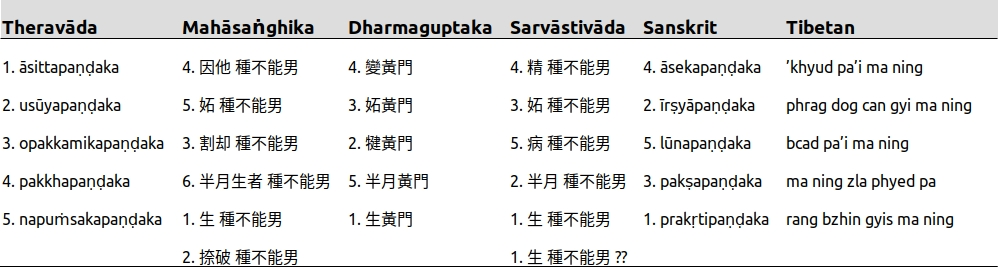
\includegraphics[width=\linewidth]{pandaka.jpg}
\label{pandaka}
\medskip

It is striking that the Dharmaguptaka Vinaya continues to describe several types of castrated men but does not equate these to {\em paṇḍaka}, while the word used for {\em paṇḍaka} is 黃門 (i.e. 'eunuch'), which is the exact definition of a castrated man.

The Theravāda and Mahīśāsaka Vinaya agree on both the background story and do not mention a list of types of {\em paṇḍaka}, but the five types of {\em paṇḍaka} are described in the commentaries. The other Vinayas all have a list of {\em paṇḍaka} who are not allowed to ordain but some of these types differ from each other or seem to have a different description. Bhikkhu Sujato\footnote{\cite{sujato2009} page 216–217.} also observes that there are various terms where "... a statement on the matter is found explicitly in all or most of the mainland Vinayas, while the Pali canon is silent, and the judgment is found in the commentary." He therefore concludes that there is an obvious explanation for this pattern, namely that the Pali is earlier.

It is therefore likely that at the time when the five types of {\em paṇḍaka} were introduced, the Theravāda and Mahīśāsaka Vinaya were already closed and therefore these five types appear in the commentarial text instead\footnote{Although the {\em Samantapāsādikā} is attributed to Buddhaghosa in the 5th century CE, this was based on earlier ones, now lost, in Prakrit and Sinhala, which were written down at the same time as the Canon, in the last century BCE. As we see here, some material in the commentaries is found in canonical texts of other schools, suggesting an early common source.}. 

The fact that the descriptions of the five terms do not always seem to match seamlessly between schools and that there is some confusion over the term 'impotent', seemingly also denoting those who are socially impaired from marriage (i.e. the concubine's son) as well as the different description of a castrated man in both the Dharmaguptaka and Mahīśāsaka Vinaya seems to point to some ambiguity as to the meaning of {\em paṇḍaka} and the inclusion of the five types could have been an attempt to resolve this.


\subsection{Development of the Paṇḍaka in the scriptures}
After having looked at the references and descriptions of the word {\em paṇḍaka} in Vedic text, Jain discussions and Buddhist scriptures in both Pali and Chinese, a clearer picture emerges of what the {\em paṇḍaka} really is and the reasons behind the Buddhist rules against ordination.

As we have seen in the previous chapter the oldest emergence of the {\em paṇḍaka} and the {\em klība} as sub-categories of the {\em napuṃsaka} ('neither male nor female') happened just after the late Vedic period. They are the 'un-males', the 'impotent', destined from birth to play a role in the larger fabric of Indian religion, society and culture. They are the embodiment of the feminine in the masculine, a living myth. They are categorised by their feminine behavior and dress, their impotence, their occupation as religious dancers and singers. They are there to remind us of the deeply ambivalent attitude of men towards women and women's sexuality, their desire for, and at the same time their fear of the feminine. Allan \cite{bomhard} points out that the word can be a loan-word from the Dravidian {\em peṇṭan, peṇṭakan, peṇṭakam}, which can mean both hermaphrodite and eunuch. This is interesting because it is clear that at least in Dravidian no difference is made between a eunuch and a hermaphrodite and I believe that the way we need to see the {\em paṇḍaka} is indeed as embodying aspects of both these terms, namely an impotent male who has female characteristics ({\em liṅga}).

As none of the words {\em paṇḍaka}, {\em klība} and {\em napuṃsaka} appear in the early Buddhist suttas and seem out of place in the Buddhist scriptures in the light of the Dhamma taught in the overall canon but are found elsewhere in Jain or other Indic texts, there is a fair chance that this does not originate from the Buddha himself. Most likely the word {\em paṇḍaka} entered the Vinaya as part of the redaction during the Second Council, especially since we have seen that this redaction played at a time when a wider religious debate with regards to the position of women in religious live was taking place. As this discussion hinged on the definition of the word {\em liṅga}, or what it means to be a 'male' or 'female', by consequence what it means to be 'neither male or female' was discussed also. The Vinaya describes the {\em paṇḍaka} as hyperlibidinous and unable to maintain his monastic precepts, which is an idea also found in the Jain texts where it is explained as the result of him possessing both male and female {\em veda}. But the Vinaya itself falls short of defining a {\em paṇḍaka} as anything else than simply hyperlibidinous and no further explanations are offered. 

\begin{figure}[!tbp]
  \begin{subfigure}{0.4\textwidth}
    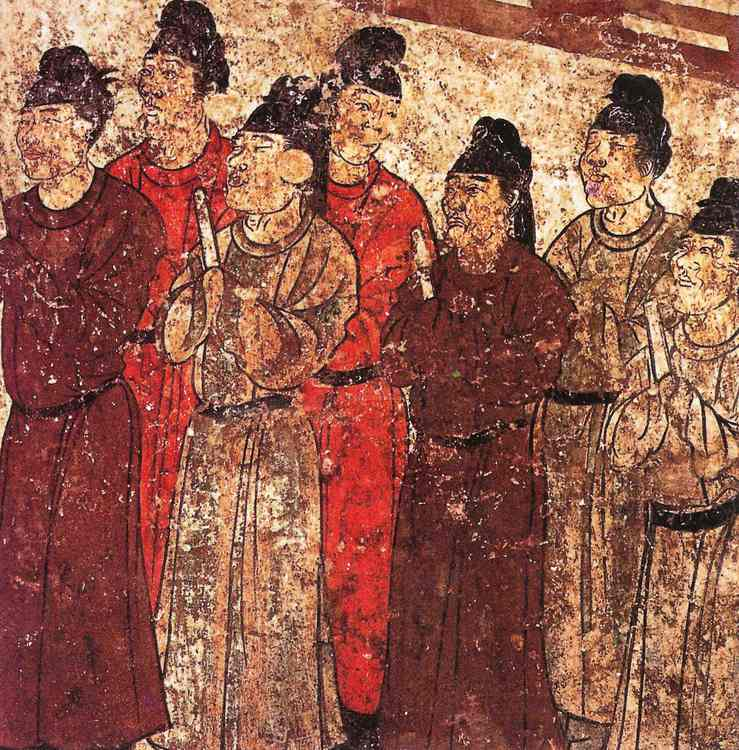
\includegraphics[width=\textwidth]{Eunuchs-in-ancient-China.jpg}
    \caption{Palace eunuchs in ancient China}
  \end{subfigure}
  \hfill
  \begin{subfigure}{0.4\textwidth}
    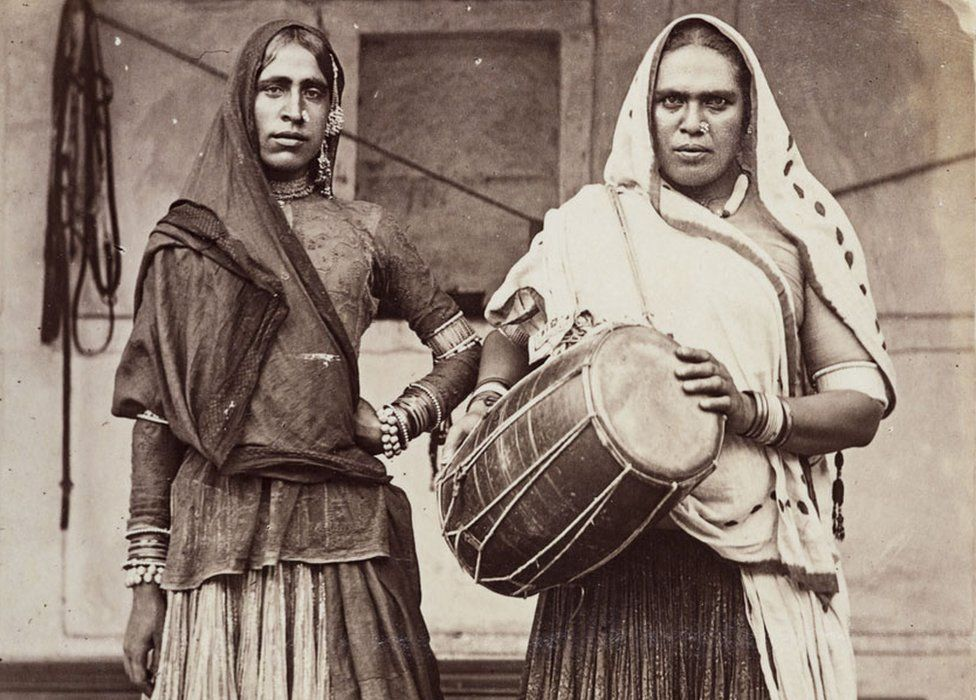
\includegraphics[width=\textwidth]{hijra.jpg}
    \caption{Hijra in India}
  \end{subfigure}
\setcounter{figure}{0}
\captionof{figure}{}
\label{eunuchs}
\end{figure}

It is in the later commentaries that we find more of a description in the form of the five types of {\em paṇḍaka}. But this also causes further confusion because the concept in its entirety did not seem to be known to the translators of the Chinese texts so they used words they knew from their own culture. There the word {\em paṇḍaka} was first translated as 'impotent' (種不能男) and later as 'eunuch' (黃門). The translation 'eunuch' however was taken from the word 'yellow gate', denoting the Han Dynasty imperial palace eunuchs. This was possibly the only way that the Chinese could relate to a {\em paṇḍaka}, being unfamiliar with the rich religious concept that they embody. It is clear that the Chinese palace eunuchs cannot be compared to the {\em hijra} from India, who are most likely the closest modern-day representative of what the {\em paṇḍakas} would have been (see figure \ref{eunuchs}).

The concept of {\em paṇḍaka} does not allow itself to be reduced to a mere word to make it acceptable and understandable for the rational mind. As Serena Nanda argues: "Whereas Westerners feel uncomfortable with the ambiguities and contradictions inherent in such in-between categories as transvestism, homosexuality, hermaphroditism, and transgenderism, and make strenuous attempts to resolve them, Hinduism not only accommodates such ambiguities, but also views them as meaningful and even powerful.\footnote{See \cite{nanda} page 20. Note that since the time Serena Nanda wrote this passage our understanding and vocabulary of sex, sexuality and gender has changed and terms like 'transvestism', 'homosexuality' and 'hermaphroditism' are no longer in use.}" It is the divine representation of the feminine within the masculine. It is the human representation of the mythical tales which have deep psychological roots, namely the ambivalence that leads to the inner struggle between man's love of the feminine and his fear thereof. The {\em paṇḍaka} does not match any contemporary notions. The closest representation of the {\em paṇḍaka} in today's world is possibly the {\em hijra}.

\section{Ubhatob­yañ­janaka}
In the Theravāda Vinaya {\em Khandhaka} 1 we find the following passage:\footnote{Khandhaka 1 Pabbajjā PTS vol 1 page 89, translation by Ajahn Brahmali.}

\begin{quote}
{\em Tena kho pana samayena aññataro ubhatobyañjanako bhikkhūsu pabbajito hoti. So karotipi kārāpetipi. Bhagavato etamatthaṃ ārocesuṃ. Ubhatobyañjanako, bhikkhave, anupasampanno na upasampādetabbo, upasampanno nāsetabboti.}
\end{quote}

\begin{quote}
At one time an {\em ubhatob­yañ­janaka} had gone forth as a monk. He had sex and made others have it. They told the Buddha and he said, “An {\em ubhatob­yañ­janaka} should not be given the full ordination. If it has been given, he should be expelled.”
\end{quote}

Just like with the {\em paṇḍaka}, the {\em ubhatob­yañ­janaka} in this passage is already ordained at the time of this incident and in a similar way we can deduce that the rule itself is limited to {\em upasampadā} (full ordination) while novice ordination is allowed, while the commentarial texts mention that both are prohibited.

For the term {\em ubhatob­yañ­janaka}\footnote{{\em Ubhato} meaning `in both ways, on both sides' and {\em byañjana} or {\em vyañjana} means `sign or mark'.} we have less material to go on as for the term {\em paṇḍaka}. It is only briefly mentioned in the Chinese Vinayas as those with two roots/faculties (二根) who are not allowed to ordain, but without any further explanation. The Therāvada Vinaya merely states that this person ``acted and was acted upon''. 

The commentarial literature is slightly more forthcoming but no less confusing as to the meaning of the word. The {\em Samantapāsādikā}\footnote{{\em Samantapādādikā}, vol. 3, para. 116 translation by Ajahn Brahmali.} states:

\begin{quote}
{\em Ubhatobyañjanako bhikkhaveti itthinimittuppādanakammato ca purisanimittuppādanakammato ca ubhato byañjanamassa atthīti ubhatobyañjanako.Karotīti purisanimittena itthīsu methunavītikkamaṃ karoti. Kārāpetīti paraṃ samādapetvā attano itthinimitte kārāpeti, so duvidho hoti – itthiubhatobyañjanako, purisaubhatobyañjanakoti.Tattha itthiubhatobyañjanakassa itthinimittaṃ pākaṭaṃ hoti, purisanimittaṃ paṭicchannaṃ. Purisaubhatobyañjanakassa purisanimittaṃ pākaṭaṃ, itthinimittaṃ paṭicchannaṃ. Itthiubhatobyañjanakassa itthīsu purisattaṃ karontassa itthinimittaṃ paṭicchannaṃ hoti, purisanimittaṃ pākaṭaṃ hoti. Purisaubhatobyañjanakassa purisānaṃ itthibhāvaṃ upagacchantassa purisanimittaṃ paṭicchannaṃ hoti, itthinimittaṃ pākaṭaṃ hoti. Itthiubhatobyañjanako sayañca gabbhaṃ gaṇhāti, parañca gaṇhāpeti. Purisaubhatobyañjanako pana sayaṃ na gaṇhāti, paraṃ gaṇhāpetīti, idametesaṃ nānākaraṇaṃ.}
\end{quote}

\begin{quote}
Because of kamma giving rise to female characteristics and kamma giving rise to male characteristics, there is for them the characteristics of both. With the male characteristic they act to transgress through sexual intercourse with women. Having encouraged another, they cause action in their own female characteristic. 

They are twofold: the female {\em ubhatob­yañ­janaka} and the male {\em ubhatob­yañ­janaka}. In regard to this, the female characteristic of the female {\em ubhatob­yañ­janaka} is apparent, but the male characteristic is hidden. The male characteristic of the male {\em ubhatob­yañ­janaka} is apparent, but the female characteristic is hidden. 

While the female {\em ubhatob­yañ­janaka} is acting with manliness among women, the female characteristic is hidden, whereas the male characteristic is apparent. 
When the male {\em ubhatob­yañ­janaka} enters the state of a woman for the sake of men, the male characteristic is hidden, whereas the female characteristic is apparent. 
The female {\em ubhatob­yañ­janaka} becomes pregnant and causes others to become pregnant. The male {\em ubhatob­yañ­janaka} does not become pregnant, but causes others to become pregnant. This is the difference between them.
\end{quote}

The Chinese equivalent of the Pali {\em Samantapāsādikā} can be found in T24 1462: 善見律毘婆沙:\footnote{T24 1462 善見律毘婆沙 0792c03–0792c06. 5\textsuperscript{th} Century CE.}
\begin{quote}
There are three kinds of two-facultied people (二根): those who can impregnate and conceive. Those who can impregnate but not conceive, and those who cannot impregnate but who can conceive. These three types of people are not allowed to become monks and take the full precepts. If they have already taken the full precepts, they should be expelled.
\end{quote}

Other Chinese commentaries have variations of the same passage:\footnote{See f.i. Shinsan X44 0744 四分律名義標釋 0450b01–0450b04.}
\begin{quote}
It is said that a person has two roots/faculties (二根): male and female. There are three kinds: The first is able to self-reproduce. He can impregnate and conceive. The second can impregnate others but cannot conceive himself. The third type cannot impregnate but he can conceive when impregnated by another. 
\end{quote}

The {\em Samantapāsādikā} identifies two types of {\em ubhatob­yañ­janakas} while the Chinese commentaries identify three. The {\em Samantapāsādikā}'s explanation is all the more puzzling because it describes the female {\em ubhatob­yañ­janaka} as having apparent female characteristics and the male characteristics hidden, but if they feel attracted to a women, they seem to be able to hide the female characteristic and make the male characteristic apparent. The opposite is described for a male {\em ubhatob­yañ­janaka}. Moreover the female {\em ubhatob­yañ­janaka} is able to become pregnant but also impregnate others so they become pregnant. This last aspect is also mentioned as one of the three types in the Chinese commentaries. The other two types in the Chinese are just described as being able to either get pregnant or impregnate others, just like females and males but with no further explanation as to why they are different from females and males. 

Apparently the ability to procreate is very important here and I would like to point out that it is humanly impossible to both conceive and impregnate.\footnote{In Appendix \ref{appendix3}, section \ref{hermaphrodite} I have described our current medical understanding of what it entails to both procreate as a male and a female.} However, as we have seen in the Vedic mythology this is a recurrent theme and there are many instances where a person is both mother and father. King Ila himself, in the form of the woman Ilā, becomes pregnant and bears a son. He/she is bound to keep on changing gender which also results in a change in sexual desires. In the {\em Mahābārata Anuśāsanaparvan}\footnote{MBh 13.12.} we find the tale of King Bhaṅgāśvana, who is longing for a son, performs a divine ritual as a result of which he gets one hundred sons but in doing so invokes the anger of the god Indra, who turns him into a woman. As a woman she conceives another hundred sons. 

Also in the Buddhist scriptures we find a similar account whereby somebody changes sex involuntarily due to their `instant kamma', triggered by impure thoughts: the story of Sorreya.\footnote{See \cite{dhammadinna} for a detailed analysis of this story that appears in the {\em Soreyyatthera-vatthu} of the {\em Dhammapada-aṭṭhavaṇṇanā}. The {\em Dhammapada-aṭṭhavaṇṇanā} was seemingly translated from Pali into Sinhalese by Buddhaghosa on the invitation of an otherwise unknown Kumārakassapa Thera. Buddhaghosa is mentioned as the author in the epilogue of this work at Dhp-a IV 235–236. Buddhaghosa lived in the 5\textsuperscript{th} Century CE. He was a commentator, translator and philosopher. He worked in the Great Monastery (Mahāvihāra) at Anurādhapura, Sri Lanka. He is also the main author of the {\em Samantapāsādikā} commentary.} The difference with the Vedic stories is that the sex-change is attributed to causality and not to a spell or curse. This shows an underlying assumption of gender inequality, namely that the male sex is preferred and the result of `good kamma', while the female sex is a result of `bad kamma'.

There are also many instances in the Vedic mythology where a gender change is a deliberate choice. Gods are able to enact a gender change in others, but also use it themselves for a variety of reasons, most notably for the purpose of sexual intercourse or to destroy male power. The gods Visnu and Śiva (see figure \ref{siva}) change sex frequently.\footnote{\cite{wendy} gives a particularly interesting account on androgyns in the ancient texts. These androgyns can have a large variety of possible characteristics and origins. See for instance pages 261–313 for detailed stories.}

It seems therefore far more likely that our elusive {\em ubhatob­yañ­janaka} is a mythological being which has no grounding in real life other than the embodiment of the feminine principle in the male. As with the {\em pakkhapaṇḍaka} (`half moon' {\em paṇḍaka}) it is not unthinkable that this was placed in the Vinaya to be complete, just under the section with the story of the mythological shape-shifting snake-turned-monk.\footnote{In various Chinese texts other shape-shifting animals are mentioned too. F.i. T85 2792 毘尼心 0667c04–0667c05 mentions dragons, fox and deer.}

The other types of {\em ubhatob­yañ­janakas} mentioned in the commentaries seem to be similar in their ability to have sex as both a male and a female, but being impotent in one of these faculties. Again, this is not something we naturally find in human beings but is a theme extensively found in the Vedic myths.

\bigskip
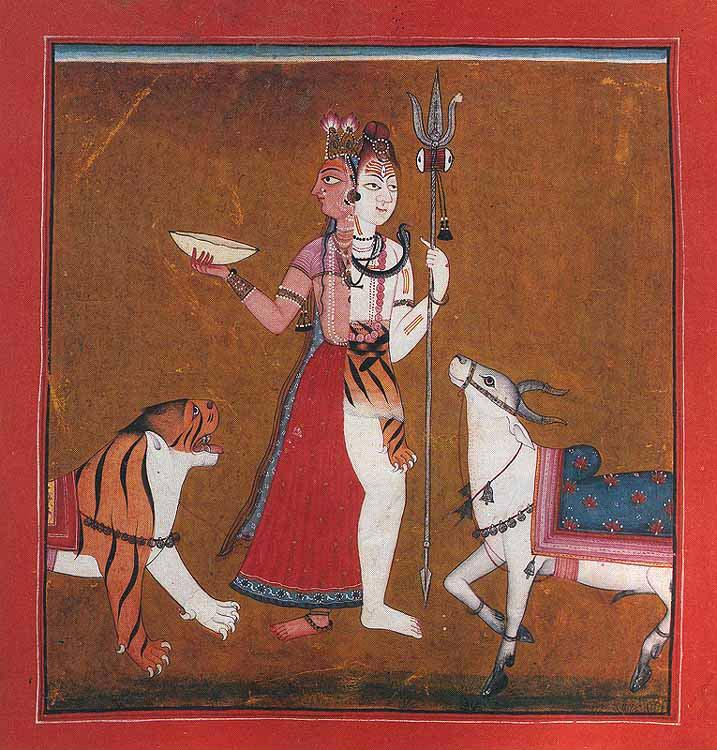
\includegraphics[width=\textwidth]{androgyne.jpg}
\begin{minipage}{\textwidth}
\captionof{figure}{Śiva in their androgynous form of Ardhanārīśwara}
\end{minipage}
\label{siva}

A story of a slightly different genre is recounted in the Buddhist {\em Dīrghāgama} Sutra T24 which describes how in the beginning all beings were male or female and were therefore subject to marriage. But the heavenly beings were bestowed with the gift to be free from marriage with no distinction between male and female and all became hermaphrodites (二根) with exactly the same faculties. This passage seems slightly different from the above because here the shift is not from male to female or visa versa but to a hermaphrodite and only bestowed on heavenly beings. So the same word 二根 is used for a hermaphrodite here but it is also seen as a great gift.

The word {\em ubhatob­yañ­janaka} does not appear in any texts outside the Buddhist Vinaya and commentaries thereof.\footnote{Appendix \ref{appendix2}, figure \ref{sanskrit1} shows that the word {\em ubhatob­yañ­janaka} does not appear in any Vedic or Brahmanical texts and only appears in the Buddhist texts. There is however another word in the {\m Varṣāvastu}, namely {\em strīpuruṣapaṇḍakam} which literally means a {\em paṇḍaka} who is both female and male.} It seems however logical that by the sheer definition of the {\em napuṃsaka} as `anything that is not entirely male' the term {\em ubhatob­yañ­janaka} also falls under this category. As a subcategory of the {\em napuṃsaka} they would have been seen as hyperlibidinous, which is in later texts explained by the fact {\em napuṃsakas} have both male and female characteristics.\footnote{As we have seen in chapter \ref{linga} it is likely that `characteristics' are defined as more than merely genital or procreative. \cite{jackson}, quoting Bunmi Methangkun (1986) (article in Thai), observes that psychological as well as physiological factors are involved in the constitution of the {\em ubhatob­yañ­janaka}. He also observes (without reference) that in early Buddhist communities men who engage in receptive anal sex are seen as feminized and thought to be hermaphrodites.} 

The term {\em paṇḍaka} as a subset of {\em napuṃsaka} was also seen as having both male and female characteristics in the Jain scriptures but is obviously not the same as {\em ubhatob­yañ­janaka}. The difference between the {\em paṇḍaka} and the {\em ubhatob­yañ­janaka} clearly seems to be on the procreative level in that the {\em ubhatob­yañ­janaka} is able to conceive and impregnate while the {\em paṇḍaka}, as an impotent man, can do neither. From the descriptions given in the {\em Samantapāsādikā} we can also conclude that the {\em ubhatob­yañ­janaka} is able to change their secondary characteristics as well as outside appearance and behaviour to appear either male or female. Again, this is not possible outside the realm of mythology.

All the Vinayas agree that the {\em ubhatob­yañ­janaka}/二根 is one of the four sex/gender types next to male, female and {\em paṇḍaka}/黃門. Considering that the male and female were seen as both having just one root/faculty (in the meaning of procreative ability), and the {\em paṇḍaka} has none\footnote{Note that when the {\em paṇḍaka} appears in the texts in the list of these four sex/gender types, it is in the Chinese Vinayas always described with the characters 黃門 (`eunuch') and never as 種不能男 (`impotent'). Indeed we find in the Chinese texts that a eunuch is somebody with the `male faculty' removed. There might be some confusion here as to what entails characteristics and the Chinese scribes would have only been able to describe this based on their own experiences in their own culture.}, the two-faculties person fills a gap. Burkhard Scherer notes that this fourfold taxonomy (`male', `female', `both ...', `neither ...') is intended to achieve the Classical Indian (and especially Buddhist) fourfold logical tetralemma called the {\em catuṣkoṭi}\footnote{See \cite{scherer} page 68 and Dr. M. Vermeulen, book on this subject is yet to be published.} and that the categories of {\em paṇḍaka} and {\em ubhatob­yañ­janaka} are largely academic. This might indeed have played a role but I believe there are also other considerations like the fact that these types are indeed found in the world, albeit in the mythology. Of course we can ask ourselves in how far the mythological beings have been created by the academic pursuits of an earlier civilization. 

Just like the term {\em paṇḍaka}, I believe that the {\em ubhatob­yañ­janaka} is a later addition to the Vinaya. The word does not appear in the early suttas\footnote{See Appendix \ref{appendix2}, figure \ref{pali1}.} and only briefly in the Vinaya. The description is so brief and hardly existent in the Chinese texts that it seems to be added almost as an after-thought. The insertion would have most likely occurred during the redaction of the Vinaya at the Second Council.

The {\em ubhatob­yañ­janaka} seems to be a rather elusive term that does not allow itself to be captured easily. Various scholars have tried to explain this as a form of intersex\footnote{For a brief description of the term `intersex' see Appendix \ref{appendix3}, section \ref{intersex}.} for the sole reason that intersex people were previously erroneously called `hermaphrodite' and a hermaphrodite can procreate in both the male and female way as is a description of the {\em ubhatob­yañ­janaka} in the commentaries. This is confusing as a true hermaphrodite does not exist among humans and is distinct from intersex. 

From the descriptions in the commentaries, the {\em ubhatob­yañ­janaka} is not human in nature. It is a mythological or heavenly being with its roots in  Vedic mythology. As Robert \cite{goldman} points out: ``... the whole phenomenon appears to be deeply bound up with a patriarchal culture's ambivalent construction of women and their sexuality.'' The Vedic stories explore the deep longing of men to be able to conceive and the idea found in a variety on Indian sources.


\section{Itthipaṇḍaka, Animittā, Nimittamattā, Vepurisikā}

There are various other words mentioned in the ordination procedures for {\em Bhikkhunīs} as described in the {\em Bhikkhunikkhandhaka} that are interesting in this context. The last three of these do not exclude an aspirant from ordination:\footnote{{\em Khandhaka} 20 {\em Bhikkhunikkhandhaka} PTS vol 2 page 271, translated by Ajahn Brahmali.} \\

\begin{tabular}{ l l }
 {\em itthipaṇḍaka} & female {\em paṇḍaka} \\
 {\em animittā } & woman who lacks genitals \\
 {\em nimittamattā } & woman with incomplete genitals \\ 
 {\em vepurisikā } & woman who is manlike \\
\end{tabular} \\

The word {\em animittā} literally means `signless' and appears a number of times in the Canon but mostly with a different meaning, namely as in {\em animitto (ceto)samādhi}, which is translated by Bhikkhu Sujato as `signless immersion', a term used in the context of meditation. In the context of not having genitals, it only appears in the Canon in the {\em Bhikkhunikkhandhaka} and as a form of abuse for women in the {\em Bhikkhu Saṁ­ghā­di­sesa­} 3; never on its own but always in the same sequence of words of which the above are a few.

The words {\em nimittamattā} and {\em vepurisikā} are explained in the {\em Samantapāsādikā}:\footnote{Sp.1.285, translations by Ajahn Brahmali.}
\begin{quote}
{\em Nimittamattāsīti tava itthinimittaṁ aparipuṇṇaṁ saññāmattamevāti vuttaṁ hoti.\\
...\\
Vepurisikāti samassudāṭhikā purisarūpā itthī.}
\end{quote}

\begin{quote}
You are a {\em nimittamattā}: you have incomplete female characteristics, merely a token.\\
...\\
{\em Vepurisikā} means a woman who has a beard and a mustache like a man.
\end{quote}

Table \ref{female} gives an overview of the terms:

\bigskip
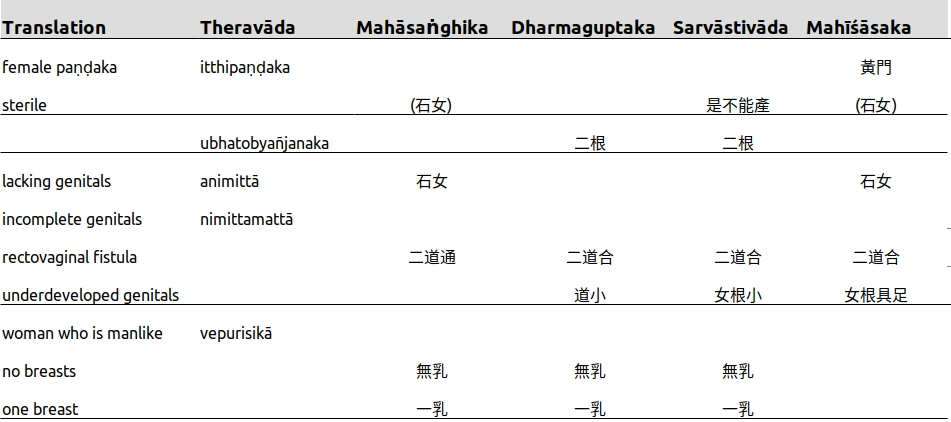
\includegraphics[width=\textwidth]{female.jpg}
\begin{minipage}{\textwidth}
\captionof{table}{The terms for gender non-conforming individuals in the {\em Bhikkhunikkhandhaka} in the various schools.}
\label{female}
\end{minipage}
\medskip

The first three of these terms in the {\em Bhikkhunikkhandhaka} are rather vague in their descriptions. The Chinese texts are not very clear on this point either but the overall questions asked here seem to be mostly to do with menstruation and diseases. At first glance it seems that the rules regarding ordination are trying to make sure that the girl in question is old enough for ordination and not ill. Rules concerning whether or not a girl has breasts can be explained as a question with regards to age, or it can be explained as a question to find out if she has developed the secondary characteristics needed or is possibly intersex. We will never know the true purpose behind these questions but it is not unlikely that these questions about the development of sexual organs were asked for the sole purpose of establishing age. After all, we also find rules in the {\em Bhikkhunīpātimokkha} that prohibit the ordination of married girls under the age of 12.\footnote{{\em Pācittiya} 65 {\em Yā pana bhikkhunī ūnad­vāda­sa­vassaṁ gihigataṁ vuṭṭhāpeyya, pācittiyaṁ.} (``Should any {\em Bhikkhunī} give acceptance to a married woman less than twelve years old, it is to be confessed.'', translation by Thanissaro Bhikkhu)} 

The question about whether a girl is sterile would point to her at least having had one child (how else would they know if she is able to conceive?) but this would seem strange if she wants to enter a celibate Order. It seems likely that the question was intended to establish if she is at least old enough to menstruate. Another possible explanation could be that women who could not conceive would be unable to marry or would be subject to divorce if the marriage remained barren. These women might have been considered outcastes and in order to survive and for protection might have sought refuge in the {\em Saṅgha}. The {\em Saṅgha} might have therefore established these rules in order to prevent them getting inundated with candidates seeking ordination for the wrong reasons.\footnote{With sincere gratitude to Ajahn Brahmali for this suggestion.} There are several stories about nuns who sought refuge in the Buddhist or Jain {\em Saṅghas} after having been rejected by their husbands or being widowed. We find some of these stories in the {\em Therīgāthā}, the Verses of the Senior Nuns, for instance in the story of {\em Isidāsī},\footnote{Thig 15.1.} {\em Candā},\footnote{Thig 5.12.} and {\em Paṭācārā},\footnote{\cite{hecker}.} or in the Jain scriptures in the story of Bhadda Kundalakesa.\footnote{\cite{hecker}.}

These terms hardly appear in any texts or commentaries. Bhikkhu \cite{sujato2009} argues that the {\em Bhikkhunikkhandhaka}, as well as other parts of the {\em Vinaya}, are a later addition, possibly dating back to the Second Council and the elusiveness of these terms seems to confirm that. 

Note that in the Pali, the word used for `characteristic' in the ordination procedure is {\em nimitta} and not {\em liṅga} or {\em vyañ­jana} as we would expect. Bhikkhu Sujato points out that the {\em Bhikkhunī} {\em Vinaya} uses its own language and terminology that is often more in line with the Jain terminology and is poorly integrated with the {\em Bhikkhu} {\em Vinaya}.\footnote{\cite{sujato2009} pages 143–145.} This could explain the discrepancies we see between the {\em Bhikkhu} and {\em Bhikkhunī} {\em Vinayas} in describing certain words pertaining to gender as used in the ordination procedures. In any case, the variability and vagueness of these terms with reference to gender do not permit a clear picture. 

It is certain though that the terms {\em paṇḍaka} and {\em ubhatob­yañ­janaka} pertained exclusively to male candidates as we have also seen in the Jain Order while the {\em Bhikkhunīs} seem to have had their own vocabulary.

There are some rare cases of people who were raised from birth as girls that later became assigned as {\em hijra} after they failed to develop secondary female sexual characteristics (breast development and menstruation) at puberty.\footnote{\cite{nanda} page 15.} Although there is very little evidence to go on, I believe that these cases could possibly be representing the {\em itthipaṇḍaka}. The term {\em itthipaṇḍaka} only appears in the Pali scriptures and in an early commentary of the {\em Mūlasarvāstivāda Vinaya} (黃門女). The latter defines the {\em itthipaṇḍaka} as either not menstruating or not having a fully formed urinal tract.\footnote{T24 1451 根本說一切有部毘奈耶雜事 0364b16 and 0364b27. With much gratitude to Dr. Hsiao-Lan Hu for pointing this out.} The Mahīśāsaka {\em Vinaya} talks about a 黃門 ({\em paṇḍaka}) without adding the character for `female' (女). We also see a similar idea emerging in Tantric Hinduisim\footnote{\cite{nanda} pages 21–22.} where a woman without menstruation is seen as a `female eunuch'.

At least for {\em Bhikkhunī} ordination in the {\em Theravāda} lineage, the characteristics of an {\em animittā, nimittamattā or vepurisikā} do not invalidate an ordination. This is possibly also true in several of the Chinese {\em Vinayas}.

\section{Changing Gender}

\begin{quote}
At one time the characteristics of a woman appeared on a monk. They told the Master. He said: “Monks, I allow that very discipleship, that very ordination, those years as a monk, to be transferred to the nuns. The monks’ offenses that are in common with the nuns are to be dealt with in the presence of the nuns. For the monks’ offenses that are not in common with the nuns, there’s no offense.”

At one time the characteristics of a man appeared on a nun. They told the Master. He said: “Monks, I allow that very discipleship, that very ordination, those years as a nun, to be transferred to the monks. The nuns’ offenses that are in common with the monks are to be dealt with in the presence of the monks. For the nuns’ offenses that are not in common with the monks, there’s no offense.”\footnote{Translation by Ajahn Brahmali, {\em Pā­rāji­ka} 1, PTS Vol. 3, page 35}
\end{quote}

In this chapter I want to pay some special attention to this very interesting passage in the Buddhist canon. The Theravāda Vinaya {\em Pā­rāji­ka} 1 describes the curious case where a monk changes gender characteristics and is now seen as a woman. She is then admitted into the Bhikkhunī order. The same holds is repeated for a nun who changes sex/gender and is from that moment on a Bhikkhu. The appearance of this passage in {\em Pārājika} 1 is a bit odd. This rule has to do with sexual intercourse and obviously a change of characteristics has nothing much to do with that. It is likely that this passage was added later. The same passage is found in several of the Chinese schools\footnote{This passage possibly appears in all of the Chinese schools but I have been unable to locate it} but in a different section, namely below the passages on ordination. This seems more logical as there is a question implied here about ordination, namely if he/she needs to re-ordain or needs a new preceptor. Again the Chinese words are confusing here, mixing up the words for 'root' and 'shape', which seem to be used as synonyms.

The Buddha seems to handle this rather curious matter in a very matter-of-fact way. The monastic in question is simply assigned in the other order while keeping their years of seniority. It does not seem to be a problem at all. He simply responds in the compassionate way we would expect.

In regards to this passage in the Vinaya Carol Anderson\footnote{See \cite{anderson2016a}} argues that this passage actually refers to the possibilty of biological sex change as well as a change of gender on the basis that both the canonical passage as the commentaries interpret the word {\em liṅga} (characteristic) to refer to both the biological sex as well as gender characteristics. The distinction between anatomical sex and culturally constructed gender is not made in pre-modern South Asia.

The most striking about the commentarial explanation\footnote{\cite{anderson2016} gives a very detailed description of this canonical passage and its commentarial explanations.} is that the change in {\em liṅga} (characteristics) happens overnight and might also revert. In fact the monastic in question can revert back and forth several times. This is something that is attributed to kamma\footnote{\cite{heirman} page 430 notes that when asleep one looses control and this can lead to shameful situations. Therefore, sexual misconduct can happen during sleep like erotic dreams or the emission of semen. Another possible explanation could be to sexual orientation. The commentaries mention that this happens when the monk is sleeping under the same roof as another monk (at least before they go to sleep) and the reverse case for a nun. If in such a case an erotic dream occurs that has to do with this other monk (/nun) i.e. homosexual attraction and the word {\em liṅga} also includes what is described as {\em veda} by the Jains, it is possible that what we have here is that this homosexual attraction is seen as a female characteristic. This is however speculation on my part and there is no proof of such a position, but it remains curious that a change of sex would happen overnight; it is far more likely that a person would suddenly find out about their homosexual sexuality overnight.}. A likely explanation of this passage is that we are dealing here with a highly academic stance with the aim of explaining something that was not well understood at the time the commentary was written. But as Carol Anderson argues, the commentarial passage can be seen as a teaching mechanism to illustrate that male characteristics are a result of good kamma in past lives while female characteristics are a result of bad kamma. This patriarchal stance is found in all Buddhist traditions so is not entirely unexpected. But it is comforting to know that at least in this passage in the canon this patriarchal stance is not found.

To conclude, we can merely say that this passage is important but also raises questions. It's position near the bottom of {\em Pārājika} 1 and in the sections on ordination in the Chinese Vinaya seem to point to a later inclusion, similar to other passages found in the Vinaya that have to do with gender non-conform individuals. In a time when Hormone Replacement Therapy and surgery were not available it does not seem to be likely that anybody just changes gender from one day to the next. One possible explanation can be found in the rare case where somebody is raised as a boy or girl but during puberty turns out to be the opposite when sex markers become more apparent. We know from the Vinaya that children were ordained very young and before puberty. But in this case this would be an intersex person. This would be an indication that intersex was not seen as an obstacle to ordination.

Although the monastic in question in this passage changes gender, they also seem to be something different from an {\em ubhatob­yañ­janaka}. After all, they are allowed to stay in robes and their change in sex/gender is not treated as anything special. This is all the more evidence that the {\em ubhatob­yañ­janaka} does not mean what we know today as intersex. The {\em ubhatob­yañ­janaka} is described as hyperlibidous and being able to change sex/gender at will for the purpose of sexual intercourse, while the monastic in this passage is obviously quite keen to stay celibate and practice as a monastic. They are also not in control of the change. The aspect of intention is important here and in the case of intersex individuals it is clear they are not intentionally so.

\section{Conclusion}
I have started my analysis by pointing out that a translation of the terms {\em paṇḍaka} and {\em ubhatob­yañ­janaka} based on a modern understanding of concepts is problematic and has led to the exclusion of transgender and intersex people from ordination.

Not only is the meaning of these terms not well understood, they have most likely been included in the Vinaya during the Second Council after the Buddha's death as the result of a wider religious debate with regards to the position of women in the Buddhist and Jain Orders, which hinged on the identification of the signs to designate somebody as a woman, which logically also led to the examination of what is male, and `neither male nor female'.

In this paper I have shown that the terms {\em paṇḍaka} and {\em ubhatob­yañ­janaka} are very likely to have deep roots in Vedic mythology and the religious enactment of that mythology by real people in sects and rituals, often involving sexual practices. The people involved in these practices were perceived as `not male' due to a combination of physical sex-characteristics and gender-expressions and were attributed with a hyperlibidinous nature due to the role they had to play in society.

Over thousands of years people in different parts of the Buddhist world have been trying to find explanations and interpretations of these words based on their own culture and society while very little research has been done as to the actual meaning of these words at the time of the Buddha and shortly thereafter as well as the influence of other Orders like the Jains. We saw that the Chinese scribes, who translated the Vinaya, could only make sense of these words using a concept they knew in that culture, namely their own imperial palace eunuchs from the Han Dynasty, a concept which is vastly different from what the term {\em paṇḍaka} is trying to convey. It would equally be a mistake for us to try and interpret these words in terms of `transgender' or `intersex', terms we are familiar with in our Western culture. The {\em paṇḍaka} and {\em ubhatob­yañ­janaka} belong in a time and place where the fabric of reality and mythology are woven into each other in a way that is daunting for our Western rational minds. For thousands of years various authors have attempted to solve the inherent ambiguities in these terms, in commentarial texts and sub-commentaries, up to the present day. The truth is that the full meaning of these terms cannot be captured in single words or phrases based on modern concepts and any interpretation of these terms will always be flawed.

The only thing we can say for certain is that the {\em paṇḍaka} and the {\em ubhatob­yañ­janaka} are seen as problematic as candidates for ordination because they are unable to keep their precept of celibacy. This is also confirmed by the Chinese commentaries\footnote{T85 2792 毘尼心 0667b25–0667c05.} as well as indicated in the origin stories. The idea that they are a threat to celibate monks because the monks might be attracted to them is not supported by the Buddhist origin stories, but could possibly be inferred from the mythological stories where shape-shifting gods seduce celibate yogis.

The main, and only, undisputed criterion for not allowing ordination to certain individuals is their difficulty in keeping the precepts. This is a fair reason for barring somebody from ordination. All criteria based on perceived or imagined sex/gender characteristics that might or might not be part of a {\em paṇḍaka} or {\em ubhatob­yañ­janaka} are not fair reasons. Transgender and intersex people are generally not hyperlibidinous and are just as able to keep the precepts as anyone else. 

It is therefore unfair, even cruel, to deny ordination to otherwise eligible individuals on the basis of a very limited and a most likely erroneous understanding of these terms, even more so because we know with a fair amount of certainty that they were inserted into the Vinaya after the Buddha's passing away, most likely influenced by discussions with other religious traditions which were held in a male patriarchal system where the fear of the feminine, and thus everything that is seen as `not-male' is paramount. The wholesome aspiration to ordain and practice in line with the Dhamma is something that needs to be encouraged, not disparaged. Ordination as a monastic is not a right to be acquired to become part of an elite group through an initiation ritual. It is to be welcomed if someone feels inspired to play a part in the propagation of the Dhamma and to help safeguard it for future generations. 

I certainly do not wish to justify ignoring any of the rules in the Vinaya. But this is an instance where contemporary social conventions are simply not covered by any of the Vinaya rules. We never before had the medical knowledge about intersex or the ability to change sex with Hormone Replacement Therapy and surgery. In such a case we must not question how to make the Vinaya rules apply to the convention, but whether such rules apply at all. And when such a rule application causes unnecessary suffering on the basis of very feeble arguments, I think it is unjust to do this. Regardless of how the Vinaya is interpreted, the doctrine of {\em anattā} (non-self), which is fundamental to all Buddhist schools, denies that there is an identity or lasting entity at the center of any being. So this makes sex and gender difference at the deepest level a superficial factor just like race, ethnicity, appearance or social status. Therefore to deny anybody ordination on the basis of this is in itself against the Dhamma.

In speaking with Buddhist monastics the question often arises as to which {\em Saṅgha}, Bhikkhus or Bhikkhunis, a transgender or intersex person should ordain into and as such also according to which ordination procedure. This question emerges from the distinct binary structure of the Buddhist institution that reflects a society vastly different from our Western one. This might have been appropriate at the time of the Buddha, but is not necessarily appropriate for our current time and place and we will have to rethink how we deal with these issues. I therefore think we should leave such questions to the individuals involved based on their gender-experience in consultation with the members of the community they wish to ordain into. The Vinaya has given us an example where the person could simply live in the {\em Saṅgha} according to their own gender-experience\footnote{PTS vol. 3 page 35. See also chapter \ref{trans}.} where they could practice in a way that was most appropriate to them in order to get the best possible opportunities to eradicate defilements and practice the teachings. As I have outlined in this article, in ancient India there was a lively debate with regards to the characteristics that make up a `man' or a `woman' and these are not so clear-cut and also not limited to primary sex/gender characteristics. There are however many variables involved and in which community a person would benefit most is not a question that is easy to answer and should be carefully considered on a case-by-case basis. 

The preservation of the religious institution and its public image is an important reason for the establishment of the Vinaya\footnote{Brenna \cite{artinger} cites Shayne Clarke, page 66.}. As Buddhism has spread across the world and across many socio-cultural environments, the challenge for the institution is to maintain its integrity while at the same time acknowledge the socio-cultural differences in the environments it operates in, the people who support it and to whom it aims to provide a refuge from suffering. Unfortunately we see all too often that people in Western cultures, already disillusioned with religion due to the scandals, misogyny and sexism in the Catholic Church, turn away from Buddhism, and therewith also from the Dhamma, because they are unable to reconcile the inclusive nature of the teachings with yet another rigid patriarchal institution that seems out of place in the modern Western world. If we are not careful in addressing these issues we will miss the ball entirely and in our aim to preserve the reputation of the {\em Saṅgha} we will lose it.

Article 1 of the UN Universal Declaration of Human Rights reads: ``All human beings are born free and equal in dignity and rights''. Denying ordination on the basis of sex or gender is against basic human rights and as Buddhists it is not only our duty to ensure the ethical standards that are expected of us in our society, but also to be the living examples of the Buddha's compassion for all beings.

\begin{quote}
As Buddhists who espouse the ideal of unconditional loving kindness and respect, judging people on their behavior instead of their birth, we should be well positioned to show leadership on the development of gender equality in the modern world and the consequent reduction of suffering for half the world’s population. Moreover, if Buddhism is to remain relevant and grow, we must address these issues head on. But how can we speak about gender equality when some of our own Theravada Buddhist organizations are gender biased? {\em Ajahn Brahmavaṃso}
\end{quote}

\section{With Gratitude}

When writing this paper I have had help and input from so many friends. It became clear to me how important this issue is for so many people and I feel very grateful that I have had the opportunity and time to dedicate to this worthwhile cause.\\

I wish to especially thank my Spiritual Advisor, Ven. Anandabodhi Bhikkhunī, who has helped me to understand my own spiritual journey as a queer female monastic in a conservative and patriarchal Buddhist {\em Saṅgha}. I also thank my good friends Ayya Yeshe Chödrön and Ven. Akāliko Bhikkhu, who have always stood by me, encouraged me to do this research and in fact are the impetus for it.\\

With regards to the practical work on this paper, I wish to express my heartfelt gratitude to Ven. Ajahn Brahmali Bhikkhu for his input, translations, discussions and feedback, to Brenna Artinger for her thorough research, to Dr. Hsiao-Lan Hu for research and feedback in regards to the Chinese texts and to Derek Sola for proofreading.\\

I feel grateful to Ven. Sujato Bhikkhu, Dr. Orna Almogi, Sebastian Nehrdich and Blake Walsh for their work on the websites \href{https://suttacentral.net/}{SuttaCentral.net} and \href{https://buddhanexus.net/}{BuddhaNexus.net}, which made research into this subject so much easier.\\

And lastly, I wish to thank all the people, and in particular the LGBTIQA+ community and other female monastics, who have supported me to live as a Bhikkhunī all these years and whose stories have touched me deeply.

\newpage
\appendix
\section{Pāli and Chinese Vinayas of the different schools}

In this chapter, I will limit myself to describing the terms as they appear in the texts in the Pāli and Chinese Vinayas of different schools and their commentaries. In the following chapters I will analyse this data to get an understanding of the history and the meanings that these texts are trying to convey.

\subsection{Theravāda Vinaya}
The {\em Theravāda Vinaya Khandhaka 1 Pabbajjā}\footnote{Pli-tv-kd 1 61} describes a {\em paṇḍaka} monk who is trying to have sex with monks and novices but is rebuked each time. He finally manages with the elephant and horse-keepers. The matter is brought to the Buddha who lays down a rule saying {\em paṇḍaka} cannot ordain and if they are already ordained they need to be expelled.

Further down there is the following passage\footnote{translation by Ajahn Brahmali}:

\begin{quote}
At one time an {\em ubhatob­yañ­janaka} had gone forth as a monk. He had sex and made others have it. They told the Buddha and he said, “An {\em ubhatob­yañ­janaka} should not be given the full ordination. If it has been given, he should be expelled.”
\end{quote}

Neither the {\em paṇḍaka} and the {\em ubhatob­yañ­janaka} are further defined here but the word {\em ubhatob­yañ­janaka} is a compound between {\em ubhato} meaning "in both ways, on both sides" and {\em byañjana} or {\em vyañjana} meaning "sign or mark".


\subsection{Mahāsaṅghika Vinaya}
The {\em Mahāsaṅghika Vinaya Bhikkhu Pakiṇṇaka} describes that monks feel groping at night and after catching the culprit, a monk, he admits being a 非男非女 i.e. neither male, nor female\footnote{T22 1425 0417c14-0418a10}. They report to the Buddha, who tells them there are six types of un-males (不能男 者有六種) (lit. those we are not capable of producing seed/impotent). The Buddha lays down a rule that none of these should be ordained and those already ordained should be expelled.

\begin{enumerate}
\item those born impotent (生). 
\item those who are born from a concubine (捺破)\footnote{This is the only place in the canon where this is mentioned but X44 0744 0432c13 mentions that there are 5 types of 黃門 (lit. yellow gate), which is translated as 'eunuch' elsewhere and 6 types of 種不能男 (i.e. seed incapable men), the 6th type being those born from a concubine}.
\item a castrated impotent man (割却), who is castrated as a punishment by the King's minister (割却 男根 lit. cut faculty of masculinity).
\item a transformed impotent man who is aroused by the touch of others but cannot ejaculate (因他)\footnote{This is a very free translation based on other texts where this type is mentioned}.
\item a jealous impotent man who is a voyeur and becomes aroused when watching others have sex (妬).
\item a 'half-moon' impotent man (半月生者) (description of what this is exactly is unclear).
\end{enumerate}

The term 非男非女 (neither male nor female) is only used by the {\em paṇḍaka} to describe himself in the this Vinaya. This could be a literal translation of the term {\em napuṃsaka} as in Vedic India this is an umbrella term of which the {\em paṇḍaka} is a subsection. The hijra of India also refer to themselves with this term.

The term 二根 (i.e. 2 roots/faculties) is mentioned in passing as a question for ordination but without further explanation. Also the term 黃門 (translated as 'eunuch'\footnote{In the remainder of this chapter I will use the translation 'eunuch' (in quotemarks) as the official translation of 黃門 according to the dictionary. I will come back to this later as I refute this translation as too narrow and probably erroneous.}) is also mentioned here without further explanation.


\subsection{Dharmaguptaka Vinaya}
In the {\em Dharmaguptaka Vinaya Pabbajja Khandhaka} the story is similar to that in the {\em Theravāda Vinaya}. A 'eunuch' (黃門) is ordained and then tries to have sex with monks and novices but is rebuked. He ends up having sex with cowherds and shepherds. The story is brought to the Buddha who lays down the rule that all 'eunuchs' have to be expelled and cannot ordain. He identifies five types of 'eunuchs'\footnote{translation by \cite{bodhi}. T22 1428 0812b23–0812c10}: 

\begin{enumerate}
\item those born as 'eunuch' (生黃門). 
\item a castrated 'eunuch' (犍黃門)\footnote{lit. a bullock-'eunuch'}.
\item a jealous 'eunuch' (妬黃門), who is aroused at the sight of others having sex.
\item a transformed 'eunuch' (變黃門). Transformed means while committing a sexual act with another, he loses masculine function, and thereby becomes a paṇḍaka.
\item a 'half-moon' 'eunuch' (半月黃門), having male function for half a month, and being impotent for the other half of the month\footnote{The word 不能男 (i.e. incapable/impotent) is used here just like in the Mahāsaṅghika Vinaya}.
\end{enumerate}

It is interesting to note that after the regular list of persons not to be ordained like animals, matricides, etc. the {\em Dharmaguptaka Vinaya} add here the story of a monk and nun resp. who change gender as is mentioned in the {\em Theravāda Pārājika 1}. The Buddha concludes that they can simply go to the other order and do not need to be expelled. The next paragraphs list the case of a monk and nun resp. who changed gender to become 男女二形 i.e. both male and female. The Buddha mentions that they have to be expelled but does not say that ordination is not possible for those who are already 男女二形 before. However we can conclude this by inference.

The {\em Dharmaguptaka Vinaya} proceeds to list details of monks who have been castrated through various causes. Obviously these are not seen as falling under the same category as the above mentioned 'eunuch'. Most of these, except for the one who self-castrates, can stay in robes; when castration happens through accident or even when it happens through karmic causes, the monk in question can remain, if he causes the castration intentionally himself he is expelled. Here the phrase is 截其 男根 (lit. cut off the male root).

While in the {\em Mahāsaṅghika Vinaya} the castration (i.e. cutting off of the male faculty 男根) is seen as an impotent man and thus not fit for ordination, here this only matters when the action is voluntary and not accidental.


\subsection{Mahīśāsaka Vinaya}
The story in the {\em Mahīśāsaka Vinaya Pabbajjā Khandhaka}\footnote{T22 1421 0117c29–0118a05} is similar to the {\em Theravāda Vinaya}. A {\em paṇḍaka} (黃門) is ordained and proceeds to try and have sex with various monks, novices and others. As a result that he is expelled together with others like him. Just like in the {\em Theravāda Vinaya}, there is no mention here of several types of {\em paṇḍaka}. At the end of the expulsion spoken by the Buddha, it is simply mentioned that the same holds true for 'two roots/faculties' (二根) without further explanation of what this is.

The story of the monk who became a woman and was allowed to live with the nuns thereafter is also mentioned here. The next paragraph is dedicated to a monk who, due to his great lust, self-castrated and as a result is expelled.


\subsection{Sarvāstivāda Vinaya}
The story in the {\em Sarvāstivāda Vinaya Pabbajjā Khandhaka}\footnote{T23 1435 0153b18–0153c17} also tells of a monk who groped other monks at night which gave problems and started rumours. Again, the Buddha identifies five types 種不能男 (impotent males). All these are not allowed to ordain and are expelled if already ordained.

\begin{enumerate}
\item those born impotent (生). (here possibly defined as a bastard)
\item a 'half-moon' impotent man (半月), who is impotent for half of the month.
\item a jealous impotent man (妬), who likes to see others engage in sex.
\item an 'essential'(?) impotent man (精), who causes others to have sex?
\item a ill impotent man who became impotent through illness (?) (病).
\end{enumerate}

In another part of the Vinaya this term 二根 (2 roots/faculties) is used next to the term 黃門 ('eunuch') but not in relation to ordination. {\em Pārājika} 1 (just like the {\em Pārājika} 1 of all the schools) mentions the existence of 4 kinds of offenders, men, women, 黃門 ('eunuch') and 二根 (2 roots/faculties). The same two words are used elsewhere in the {\em Sarvāstivāda Vinaya} while the word 種不能男 (impotent) is only used in the list for those who cannot ordain.


\subsection{Commentaries}

Going beyond the Vinaya itself into the commentarial scriptures, we find the following in the {\em Theravāda Mahāvagga-aṭṭhakathā} to explain more about the nature of these two classes. It defines five types of {\em paṇḍaka}\footnote{The {\em Samantapāsādikā}: Vol. V, p. 1015f. is a translation of Sinhala commentaries into Theravāda by Bhikkhu Buddhaghosa in the 5th century CE. It was based on the Mahāpaccariya and the Kurundī Atthakathā. See \cite{goonesekere} for details on Theravāda Commentaries}\footnote{Following translations/explanations as in \cite{bomhard} and \cite{thanissaro}}:

\begin{enumerate}
\item {\em āsittapaṇḍaka}: a man who gains satisfaction from performing oral sex on another man and from swallowing his semen or who only becomes sexually aroused after swallowing another man’s semen. 
\item {\em usūyapaṇḍaka}: a voyeur, that is, a person who gains sexual satisfaction from watching others have sex. 
\item {\em opakkamikapaṇḍaka}: eunuch, due to castration.
\item {\em pakkhapaṇḍaka}: those who become sexually aroused in parallel with the phases of the moon\footnote{According to \cite{bomhard}, the term pakkhapaṇḍaka (Skt. {\em pakṣapaṇḍaka}) probably does not refer, as traditionally understood, to an individual who becomes sexually aroused parallel to the phases of the moon, i.e., to someone who is aroused during the fortnight of either the waxing or waning moon, but to someone “who acts wrongly sexually, who behaves badly sexually.” He hypothesizes that {\em pakkha} of the compound {\em pakkhapaṇḍaka} should be understood in terms of its alternative meaning “a cripple,” and that the corresponding Sanskrit should not be understood as {\em pakṣa} but rather {\em phakka} (“cripple,” adj. “lame, crippled, maimed”), derived from the Skt. verbal root {\em phakk}, (a) “to creep, to steal along; (b) to have a preconceived opinion; (c) to act wrongly, to behave badly.” He thus considers the third meaning of phakk as most relevant to the case at hand.}.
\item {\em napuṁsakapaṇḍaka}: a person born without sexual organs. 
\end{enumerate}

It is interesting to note that here not all {\em paṇḍaka} are barred from ordination, in contrast to what the Vinaya mentions. Only the last three types are forbidden to ordain\footnote{\cite{wong} and \cite{thanissaro}}.

The Chinese commentarial texts add that these five cannot ordain because they have difficulty keeping the precepts\footnote{T85 2792 毘尼心 0667b25-0667b26}.

For the {\em ubhatob­yañ­janaka} we find the following\footnote{translation by Ajahn Brahmali}:

\begin{quote}
Because of kamma giving rise to female characteristics and kamma giving rise to male characteristics, there is for them the characteristics of both. With the male characteristic they act to transgress through sexual intercourse with women. Having encouraged another, they cause action in their own female characteristic. 

They are twofold: the female {\em ubhatob­yañ­janaka} and the male {\em ubhatob­yañ­janaka}. In regard to this, the female characteristic of the female {\em ubhatob­yañ­janaka} is apparent, but the male characteristic is hidden. The male characteristic of the male {\em ubhatob­yañ­janaka} is apparent, but the female characteristic is hidden. 

While the female {\em ubhatob­yañ­janaka} is acting with manliness among women, the female characteristic is hidden, whereas the male characteristic is apparent. 
When the male {\em ubhatob­yañ­janaka} enters the state of a woman for the sake of men, the male characteristic is hidden, whereas the female characteristic is apparent. 
The female {\em ubhatob­yañ­janaka} becomes pregnant and causes others to become pregnant. The male {\em ubhatob­yañ­janaka} does not become pregnant, but causes others to become pregnant. This is the difference between them."
\end{quote}

The Chinese equivalent of the {\em Samantapāsādikā} can be found in T24 1462: 善見律毘婆沙\footnote{T24 1462 0792c03–0792c06. 5th century CE}:
\begin{quote}
There are three kinds of 2-facultied people (二根): those who can impregnate and conceive; those who can impregnate but not conceive; and those who cannot impregnate but who can conceive. These three types of people are not allowed to become monks and take the full precepts; if they have already taken the full precepts, they should be expelled.
\end{quote}

Other Chinese commentaries have variations of he same passage. For instance Shinsan X44 0744 0450b01–0450b04 mentions:
\begin{quote}
It is said that a person has two roots/faculties (二根): male and female. There are three kinds: The first is able to self-reproduce. He can impregnate and conceive. The second can impregnate others but cannot conceive himself. The third type cannot impregnate but he can conceive when impregnated by another. 
\end{quote}


\newpage
\section{Appendix 2: Word frequency}
\label{appendix2}

The following charts show how often some of the words are used in the Pali canon as well as in the Sanskrit and Tibetan texts. Note that the size of the specific parts of the canon is not taken into account so we have to be careful drawing definate conclusions from these charts, but they do show the relative importance of these words. 

\subsection{Pali canon and commentaries}

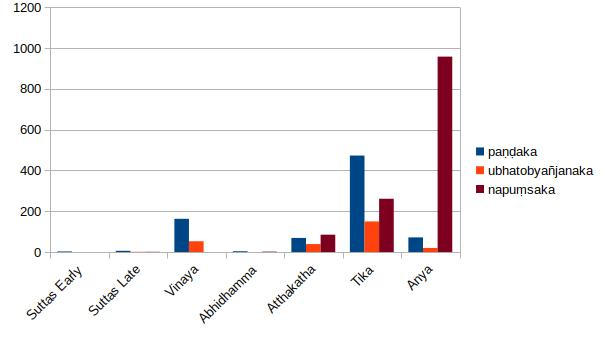
\includegraphics[width=\linewidth]{pali.jpg}
\captionof{figure}{Frequency of words in the pali canon and commentaries}
\label{pali1}

\subsection{Sanskrit Buddhist and Vedic canon}

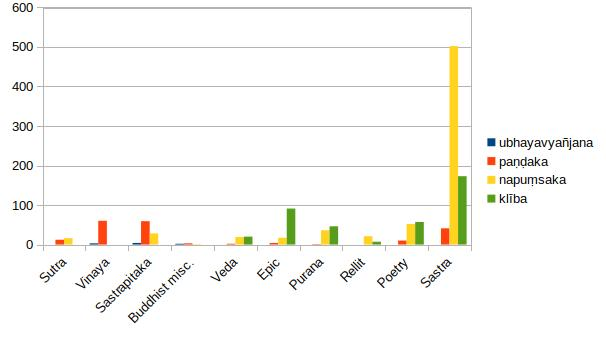
\includegraphics[width=\linewidth]{sanskrit.jpg}
\captionof{figure}{Frequency of words in the Sanskrit Buddhist and Vedic canon}
\label{sanskrit1}

\medskip
It is important to note that unlike the texts in the Pali canon, the search over the Sanskrit text only use the GRETIL database and do not comprise of the entire Buddhist canon. The Vedic canon is also included in this chart.


\subsection{Tibetan canon and commentaries}

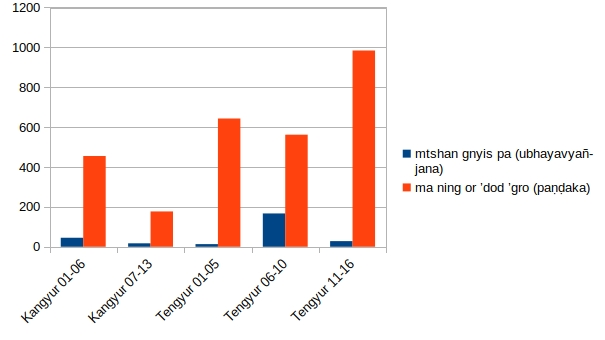
\includegraphics[width=\linewidth]{tibetan.jpg}
\captionof{figure}{Frequency of words in the tibetan canon and commentaries}
\label{tibetan1}



\newpage
\section{Appendix 1: Glossary of Definitions}
\label{appendix1}

\subsection{Definitions of Pāli words}
In this section I refer to the various dictionary definitions of the words relevant to the subject matter and provide links to these dictionaries.

\subsubsection{Napuṃsaka}
Pāli word: {\em napuṃsaka} \\
Pāli dictionary: \href{https://suttacentral.net/define/napu%E1%B9%83saka}{see SuttaCentral} \\
Sanskrit word: {\em napuṃsaka} \\
Sanskrit dictionary: \href{https://www.wisdomlib.org/definition/napumsaka}{see WisdomLib} \\

\subsubsection{Paṇḍaka}
Pāli word: {\em paṇḍaka} \\
Pāli dictionary: \href{https://suttacentral.net/define/pa%E1%B9%87%E1%B8%8Daka}{see SuttaCentral} \\
Sanskrit word: {\em paṇḍaka} \\
Tibetan word: {\em ma ning} or {\em ’dod ’gro} \\
Chinese word: {\em 種不能男} or {\em 黃門} (first one lit means 'neither male nor female'.\\
ITLR dictionary: \href{http://www.itlr.net/hwid:281142}{see itlr.net} \\

\subsubsection{Ubhatob­yañ­janaka}
Pāli word: {\em ubhatob­yañ­janaka} or {\em ubhatovyañ­janaka} \\
Pāli dictionary: \href{https://suttacentral.net/define/ubhatovya%C3%B1janaka}{see SuttaCentral} \\
Sanskrit word: {\em ubhayavyañjana} \\
Tibetan word: {\em mtshan gnyis pa} \\
ITLR dictionary: \href{http://www.itlr.net/hwid:62844}{see itlr.net} \\

\subsubsection{Other references}
There are various other words mentioned in the ordination procedures for Bhikkhunī as described in Bhikkhunikkhandhaka that might be interesting in this context. These do not excluse from ordination and have been translated by Ajahn Brahmali as follows: \\

\begin{tabular}{ l l }
 {\em animittā } & woman who lacks genitals \\
 {\em nimittamattā } & woman with incomplete genitals \\ 
 {\em vepurisikā } & woman who is manlike \\
\end{tabular} \\

The word {\em animittā} literally means 'signless' and appears a number of times in the canon (excluding commentaries) but mostly in a different meaning, namely as in {\em Animitto (ceto)samādhi}, which is translated by Bhikkhu Sujato as 'signless immersion', a term used in the context of meditation. In the context of not having genitals, it only appears in the canon in the Bhikkhunikkhandhaka and as a form of abuse for women in the Bhikkhu Saṃ­ghā­di­sesa­ 3, never on it's own but always in the same sequence of words of which the above are a few. This points towards a later development.


\subsection{Modern Definitions}
In this section I list a few terms relevant to the subject matter because there are many misunderstandings with regards to these terms and their meanings. For other terms, I refer to \href{https://www.hrc.org/resources/glossary-of-terms}{the website of the Human Rights Campaign}

\subsubsection{Intersex}
\label{intersex}
The definition of the term 'intersex' according to the \href{https://unfe.org/system/unfe-65-Intersex_Factsheet_ENGLISH.pdf}{UN Office of the High Commissioner for Human Rights} is as follows:

\begin{quote}
Intersex people are born with sex characteristics (including genitals, gonads and chromosome patterns) that do not fit typical binary notions of male or female bodies.

Intersex is an umbrella term used to describe a wide range of natural bodily variations. In some cases, intersex traits are visible at birth while in others, they are not apparent until puberty. Some chromosomal intersex variations may not be physically apparent at all.
\end{quote}

Intersex can be divided into 4 categories according to the \href{https://medlineplus.gov/ency/article/001669.htm}{US National Library of Medicine}:

\begin{tabular}{ l l }
46, XX intersex & female internal organs and chromosomes \\
& external genitals appear male \\
46, XY intersex & male internal organs and chromosomes \\
& external genitals appear female or ambiguous \\
True gonadal intersex & both ovarian and testicular tissue \\
& external genitals ambiguous or \\
& appear female or male \\
Complex or undetermined intersex & chromosomes discrepancies only \\
\end{tabular}


\subsubsection{Hermaphrodite}
\label{hermaphrodite}
A hermaphrodite is an organism that has both male and female reproductive organs. Until the mid-20th century, 'hermaphrodite' was used synonymously with 'intersex'. The distinctions 'male pseudohermaphrodite', 'female pseudohermaphrodite' and especially 'true hermaphrodite' are terms no longer used, which reflected histology (microscopic appearance) of the gonads. Medical terminology has shifted not only due to concerns about language, but also a shift to understandings based on genetics.

Currently, hermaphroditism is not to be confused with intersex, as the former refers only to a specific phenotypical presentation of sex organs and the latter to a more complex combination of phenotypical and genotypical presentation. Using hermaphrodite to refer to intersex individuals is considered to be stigmatizing and misleading\footnote{See \href{https://web.archive.org/web/20130701061246/http://www.isna.org/faq/hermaphrodite}{Intersex Society of North America}}. Hermaphrodite is used for animal and plant species in which the possession of both ovaries and testes is either serial or concurrent, and for living organisms without such gonads but present binary form of reproduction, which is part of the typical life history of those species; intersex has come to be used when this is not the case.

\subsubsection{Transgender}
Transgender people have a gender identity or gender expression that differs from the sex that they are assigned at birth (\cite{altilio}). Some transgender people who desire medical assistance to transition from one sex to another identify as transsexual (\cite{polly}). Transgender, often shortened as trans, is also an umbrella term. In addition to including people whose gender identity is the opposite of their assigned sex (trans men and trans women), it may include people who are not exclusively masculine or feminine (people who are non-binary or genderqueer, including bigender, pangender, genderfluid, or agender). Other definitions of transgender also include people who belong to a third gender, or else conceptualize transgender people as a third gender.

The term transgender is also distinguished from intersex. 

The opposite of transgender is cisgender, which describes persons whose gender identity or expression matches their assigned sex.

Many transgender people experience gender dysphoria, and some seek medical treatments such as hormone replacement therapy, sex reassignment surgery, or psychotherapy. Not all transgender people desire these treatments, and some cannot undergo them for financial or medical reasons. (\cite{maizes})



\newpage
\bibliographystyle{plainnat}
\bibliography{bib}


\end{document}

